% !TeX spellcheck = it_IT
\title{Algoritmi e Complessità}
\author{Massimo Perego}
\date{}

\documentclass[11pt]{article}
\usepackage{enumitem} 					%enumerate, itemize
\usepackage{graphicx} 					%File grafici 
\usepackage{xcolor}
\usepackage{listings}
\usepackage{amsmath}  					%Roba Matematica
\usepackage{amssymb}
\usepackage{amsfonts}
\usepackage{mathtools}
\usepackage{gensymb}  					%Simboli vari 
%\usepackage{pgfplots} 					%Grafici
\usepackage{texdate} 					%Data formattata, usare \printfdate{ISOext}
\usepackage[hidelinks]{hyperref} 			%link
\usepackage[english]{babel} 				%Selezione lingua per il documento
\usepackage[autostyle, english = american]{csquotes} 	%Virgolette che si aprono/chiudono da sole
\usepackage[font={small}]{caption} 			%Font caption immagini ridotto
\usepackage[utf8]{inputenc} 				%Traduzione input
%\usepackage{fancyhdr} 					%Controllo per headers e footers
\usepackage[parfill]{parskip} 				%A capo niente spazio
\usepackage{float}
%\usetikzlibrary{datavisualization} 			%Grafici
%\usetikzlibrary{datavisualization.formats.functions}
\MakeOuterQuote{"}
%\DeclareMathOperator{\sgn}{sgn}			%sgn operator
\lstset{basicstyle=\ttfamily,language=c,keywordstyle=\color{blue}, showstringspaces=false} %Command is \begin{lstlisting}

\usepackage{amsthm}
\usepackage{algorithm}
\usepackage{algorithmic}

\DeclareMathOperator*{\opt}{opt}

\begin{document}
	\initcurrdate
	\maketitle 									%Titolo 
	\setlist[itemize]{noitemsep} 							%Meno spazio in liste itemize
	\setlist[enumerate]{noitemsep} 							%Meno spazio in liste enumerate
	\newcommand{\nn}{\hfill \\}
	%\newcommand{\RNum}[1]{\uppercase\expandafter{\romannumeral #1\relax}} 		%Numeri romani
	%\newcommand{\myfont}{\fontfamily{lmtt}\selectfont } 				%Font BDD
	%\newcommand{\notimplies}{\;\not\!\!\!\implies} %Comando not implies corretto
	%\newcommand{\ts}{\hspace*{0.666cm}}
	
	\tableofcontents
	
	\newpage
	
	\section{Notazione}
	%Controlla slide, c'è un $\epsilon$ che manca
	
	Definire una notazione che verrà usata da qui in avanti. \\
	
	Verranno usati tanto gli \textbf{insiemi}: $\mathbb{N}$, $\mathbb{Z}$, $\mathbb{Q}$, $\mathbb{R}$ ed anche le versioni con \textbf{solo i positivi} di ognuno di questi $\mathbb{N}^+$, ... \\
	
	Un \textbf{magma} è un \textbf{insieme più un'operazione binaria} definita su di esso. Esempio
	$$ (A, \circledast) $$
	
	Se il magma ha la \textbf{proprietà associativa} sull'operazione è un \textbf{semigruppo}
	$$ (y \circledast z) \circledast x = y \circledast (z \circledast x) $$
	
	Se \textbf{esiste elemento neutro} rispetto all'operazione si parla di \textbf{monoide}. Se esiste elemento neutro è unico
	$$ x \circledast \overline{\epsilon} = \overline{\epsilon} \circledast x = x $$
	
	Se l'\textbf{operazione è anche commutativa} allora \textbf{monoide abelliano}. L'esempio più semplice sono i naturali con l'operazione somma. \\
	
	Se per ogni elemento c'è \textbf{anche un inverso} allora è un \textbf{gruppo}. \\
	
	Definendo un \textbf{alfabeto come un insieme finito non vuoto} di elementi. \\
	
	\paragraph{Monoide libero:} prendendo un alfabeto $\Sigma$ e considerando tutte le sequenze finite costituite da elementi dell'alfabeto, si nota con 
	$$w \in \Sigma^{\ast} \;\;\; w = w_1, w_2, w_3, ... , w_n \;\;\;\; n \geq 0 \;\;\;$$
	$$ w_i \in \Sigma \;\;\;\;\;\; |w| = n$$
	
	\newpage
	
	La concatenazione è un'operazione interna a $\Sigma^{\ast}$, due parole se le concateno le metto una dopo l'altra
	$$ w = w_1, w_2, w_3, ... , w_n $$ 
	$$ w' = w_1', w_2', w_3', ... , w_m' $$ 
	$$ w \cdot w' = w_1, w_2, w_3, ... , w_n, w_1', w_2', w_3', ... , w_m'  $$
	
	$(\Sigma^\ast, \cdot)$ è un monoide, chiamato \textbf{monoide libero} su $\Sigma$ (abelliano solo quando nell'insieme è presente solo una lettera). \\
	
	In generale un monoide libero è un monoide con una base, ovvero un insieme di elementi che generano il monoide e che non possono essere generati da altri elementi della base.\\
	
	Se $A$ e $B$ sono due insiemi allora $B^A$ è l'\textbf{insieme delle funzioni da $A$ a $B$}
	$$ B^A = \{f | f : A \rightarrow B\}$$
	
	La cardinalità finale è quella di $|B|^{|A|}$, per questo la notazione è in quest'ordine.\\
	
	Con l'\textbf{insieme} $K$ si intende 
	$$ K = \{0, 1, \, ... \, , k-1\}$$
	Con $0$ che significa l'insieme vuoto.\\
	
	Sostanzialmente l'insieme di tutti i valori inferiori a $K$.\\
	L'insieme dei valori dei bit si chiama $2 = \{0,1\}$.\\
	
	Considerando
	$$ 2^A = \{f | f : A \rightarrow 2\} = \{f | f : A \rightarrow \{0,1\}\}$$
	Questa è una funzione che \textbf{mappa ogni elemento di $A$ in $0$ o in $1$}, in biezione con $\cong \{x | x \text{ è sottoinsieme di } A\} = P(A)$ (insieme delle parti di $A$).\\
	
	\newpage
	
	$A^2$, \textbf{insieme delle coppie di elementi di $A$}, ma sarebbe 
	$$ A^2 = \{f | f : 2 \rightarrow A\} = \{f|f : \{0,1\} \rightarrow A\} $$
	che è in biezione con
	$$ A \times A $$
	Quindi con il prodotto cartesiano di $A$ con $A$.\\
	
	$2^\ast$ è un monoide libero sull'alfabeto binario, \textbf{tutte le combinazioni binarie}. Quindi una qualsiasi stringa in binario sarà parte di questo monoide.\\
	
	Mentre $2^{2^\ast}$ rappresenta la \textbf{famiglia di tutti i linguaggi binari} (su $\{0,1\}$).\\
	Ogni linguaggio che consiste di numeri binari è membro di $2^{2^\ast}$.\\
	
	\newpage
	
	\section{Algoritmi 101}
	
	\subsection{Cos'è un problema?} 
	
	Un \textbf{problema} $\pi$ è \textbf{costituito da}:
	\begin{itemize}
		\item Un \textbf{insieme di input} possibili $I_\pi$
		
		\item Un \textbf{insieme di output} possibili $O_\pi$
		
		\item Funzione $Sol_\pi: I_\pi \rightarrow 2^{O_\pi} \setminus \{\emptyset\}$ \textbf{mappa ogni input ad un insieme di output corretti possibili}, non è detto che dobbiamo avere un solo output corretto, possono esserci più output validi. Molti problemi considerati potranno avere più output corretti.
	\end{itemize}
	
	\paragraph{Esempio di problema:} Descrizione informale: decidere se un numero è primo. \\
	
	Supponendo che si tratta, in input, di numeri naturali scritti in base $2$ (non specificato, da specificare, questo sono assunzioni).\\
	Mentre in output si può avere solo $sì$ o $no$, si tratta di un problema di decisione
	$$ O_\pi = \{no, yes\} $$
	
	Anche se non esplicitamente detti, \textbf{input e output dovrebbero essere specificati come su un linguaggio binario}, sono \textbf{sequenze di bit}.\\
	
	\newpage
	
	\paragraph{Altro esempio:} emettere il MCD tra due interi positivi $x$ e $y$. Non è più un problema di decisione.\\
	
	Come distinguo i due valori in input?  \\
	
	Soluzioni: raddoppio tutti i bit e $01$ diventa il separatore. \\
	
	Altra soluzione: Elias $\gamma_x$ sapendo la lunghezza $l$ in bit dell'input $x$, scrivo $l$ in unario, quindi $l$ bit ed uno $0$ prima dell'input, così in base a quanti 1 leggo so quanti bit leggere dopo.  \\
	
	I problemi generalmente saranno scritti "approssimativamente", quindi sono necessarie diverse assunzioni per specificarli formalmente.\\
	
	Nella pratica quindi i dettagli di implementazione dell'algoritmo cambieranno, ma tra $n^2$ e $n^2 \log n$ ci cambia poco, sempre dominato da un polinomio ed un polinomio vale l'altro (assunzione solo teorica, nella realtà non è proprio così ma sticazzi).
	
	\newpage
	
	\subsection{Cos'è un algoritmo?}
	Senza definirlo esattamente in modo formale, si presume che a questo punto tu ne abbia un'idea.\\
	
	Ma se proprio dobbiamo: tutti gli algoritmi sono Macchine di Turing (programmi eseguibili da una MdT). \\
	
	\paragraph{Tesi di Church-Turing:} storicamente, hanno preso tutte le definizioni di algoritmi presenti, hanno provato che sono tutte equivalenti ed ogni definizione riporta alla stessa famiglia di problemi risolvibili: problemi che con una MdT sono risolvibili allora sono risolvibili anche secondo qualsiasi altra definizione.\\
	
	Al giorno d'oggi è importante perché si traspone in "ogni linguaggio di programmazione (Turing-completo) può risolvere gli stessi problemi risolvibili da tutti gli altri". 
	
	In passato è stato discusso come sia impossibile concepire una definizione realistica di algoritmo non equivalente alla MdT.\\
	
	\newpage
	
	\subsection{Cos'è un algoritmo per un problema $\pi$?}
	
	Dando $x \in I_\pi$ ad un algoritmo $A$ eseguito su una MdT restituirà $y \in O_\pi$ tale che $y \in Sol_\pi (x)$, ovvero \textbf{dato un input restituisce una soluzione tra quelle ammesse}.\\
	
	\textbf{Molti problemi non sono risolvibili}. Considerando i problemi di decisione, data una stringa binaria bisogna rispondere $sì$ o $no$.\\
	
	Se ne può avere uno per ogni possibile insieme di stringhe binarie, gli elementi di $2^{2^\ast}$ sono tutti problemi di decisione, e possiamo vedere che
	$$ |2^{2^\ast}| \cong |2^{\mathbb{N}}| \cong |\mathbb{R}|$$
	ha la potenza del continuo, quindi il numero possibile di problemi di decisione è un infinito non numerabile. \\
	
	Ma i programmi (algoritmi per risolvere questi problemi) sono infiniti? Sì, ma hanno cardinalità $|\mathbb{N}|$, essendo questa la dimensione dell'insieme di risposte possibili ($|2^\ast|$).\\
	
	Quindi \textbf{i problemi sono di più dei possibili programmi per risolverli}. Per forza di cose la maggior parte dei problemi non sono risolvibili. \\
	
	\newpage
	
	\subsection{Teoria della complessità}
	Tutti i problemi che verranno considerati sono risolvibili, ma \textbf{quanto efficientemente}? La teoria della complessità stabilisce la \textbf{quantità di risorse consumate da un problema}.
	
	Si può parlare di teoria della complessità in due termini:
	\begin{itemize}
		\item \textbf{Algoritmica}
		\item \textbf{Strutturale}
	\end{itemize}
	
	
	\subsubsection{Algoritmica}
	
	Dato $\pi$
	\begin{enumerate}
		\item Stabilire \textbf{se è risolvibile} (per noi sempre sì); c'è un algoritmo che lo risolve?
		
		\item \textbf{Risolvibile con che costo?} Ci sono più \textbf{misure} possibili:
		\begin{itemize}
			\item Tempo (solitamente sarà usata questa)
			\item Spazio
			\item Numero di processori utilizzati/somma dei tempi di tutte le CPU
			\item Energia dissipata
		\end{itemize}
	\end{enumerate}
	
	Considerando il tempo, vogliamo stabilire \textbf{dato un input quanto tempo impiega}, ovvero \textbf{quanti passi} deve svolgere
	$$ T_A : I_\pi \rightarrow \mathbb{N}$$
	
	Invece di calcolare la \textbf{complessità} input per input si considera "per taglia", \textbf{per ogni dimensione}, prendendo l'input che ci impiega il tempo massimo per taglia
	$$ t_a : \mathbb{N} \rightarrow \mathbb{N}$$
	$$ t_a (n) = \max \{T_A (x) \, | \, x \in I_\pi \text{ t.c. } |x| = n\} $$
	
	Si tratta di un'assunzione worst-case, dati input di stessa dimensione prendo il peggiore. Potrebbe essere utile fare una media al posto di un'assunzione pessimistica, ma noi teniamo così perché è comodo, inoltre nella realtà possiamo solo metterci di meno.\\
	
	\newpage
	
	Se dobbiamo valutare quale algoritmo usare il \textbf{confronto va fatto asintoticamente}, i casi piccoli sono "facili" (di solito, ma andrebbero considerati i casi d'uso effettivi? In estremo potrei fare una tabella). Quindi consideriamo come le performance dell'algoritmo scalano con la dimensione dell'input.\\
	
	Quindi due assunzioni: worst-case e asintotico. \\
	
	Generalmente quindi tra
	$$ t_a = O (n^2) \;\;\;\;\;\; t_a = O(n^7)$$
	meglio il primo tendenzialmente.
	
	Bisogna anche provare che non ci possono essere cose migliori/peggio, quindi upper and lower bound.\\

	\newpage
	
	\subsubsection{Strutturale}
	
	Fissato un problema $\pi$, qual'è la sua complessità? Non vogliamo cercare la complessità di un algoritmo, ma la \textbf{complessità del miglior algoritmo che risolve un problema} $\pi$. Questo permette di eliminare facilmente problemi che non hanno soluzioni efficienti.\\
	
	Con la notazione worst case asintotica sopracitata possiamo avere un \textbf{upper bound} per il \textbf{tempo impiegato} per la risoluzione di un problema. Quindi nel caso peggiore avrà asintoticamente quel comportamento. $O(n^2)$ vuol dire che nel caso peggiore ci mette tempo quadratico rispetto all'input.\\
	
	Esistono anche \textbf{lower bounds}, ovvero limiti inferiori per il \textbf{tempo impiegato} da un algoritmo e dimostrarlo implica \textbf{dimostrare che per come è fatto un problema, questo non può impiegare meno di un certo tempo}. $\Omega(n)$ vuol dire che non ci può mettere meno di tempo lineare.\\
	
	Un problema viene "chiuso" quando upper e lower bound coincidono, vuol dire che si ha l'algoritmo ottimo e si conosce esattamente la complessità del problema. Per esempio, l'ordinamento di array basato su confronti e scambi ci mette esattamente $n \log n$, quindi si dice $\Theta(n \log n)$.\\
	
	Le casistiche problematiche sono quando gli \textbf{upper bound sono esponenziali ed i lower bound polinomiali}, quindi le possibilità sono: 
	\begin{itemize}
		\item esiste un upper bound da migliorare, quindi esistono algoritmi polinomiale non ancora scoperti
		\item esiste un lower bound esponenziale, quindi il problema non è risolvibile in tempo polinomiale
	\end{itemize}
	
	In entrambi i casi saremmo contenti, il non avere informazioni a riguardo è il problema.\\
	
	\newpage
	
	\subsubsection{Classi di complessità:} 
	
	Per la complessità strutturale sono state inventate delle classi di problemi per \textbf{dividerli in base alla difficoltà di risoluzione}: 
	\begin{itemize}
		\item $\mathcal{P}$: problemi di decisione risolvibili in tempo polinomiale; la domanda diventa "il mio $\pi$ è in $\mathcal{P}$?"
		\item $\mathcal{NP}$: problemi di decisione risolvibili in tempo polinomiale \textbf{su macchine non deterministiche} 
	\end{itemize}
	
	Sostanzialmente macchine non deterministiche vuol dire che: una macchina su cui il programma può essere eseguito più volte in parallelo con determinate variabili settate a 0 e 1, permettendo di eseguire in parallelo tante "versioni" ed ottenere una soluzione per ogni esecuzione parallela. La soluzione alla fine è \textit{yes} se esiste almeno una esecuzione che ha dato \textit{yes} e \textit{no} se tutte le esecuzioni hanno riportato \textit{no}. \\
	
	\paragraph{CNF-Sat problem:} l'input è una espressione logica in forma CNF (Conjunctive Normal Form), quindi un \texttt{and} tra clausole, ognuna delle quali contiene \texttt{or} di letterali, i quali possono essere variabili o negazioni di variabili.\\
	
	L'output è se l'espressione logica $\varphi$ è soddisfacibile, ovvero, esiste $\exists$ assegnazione che rende $\varphi$ \textit{true}? \\
	Attualmente questo problema si pensa sia in $\mathcal{NP}$, non sappiamo se possa stare in $\mathcal{P}$.\\
	
	Sappiamo rientra in $\mathcal{NP}$ perché è facile pensare ad un algoritmo non deterministico per questo problema, basta avere una esecuzione parallela per ogni possibile valore di ognuna delle variabili, e se almeno un output è \textit{sì} allora è soddisfacibile.\\
	
	\newpage
	
	\paragraph{Relazione tra $\mathcal{P}$ e $\mathcal{NP}$:} $\mathcal{P}$ è ovviamente \textbf{incluso in} $\mathcal{NP}$, dato che se posso risolvere un problema in modo polinomiale, posso risolverlo anche con il parallelismo aggiunto delle macchine non deterministiche.\\
	
	La vera domanda è se $\mathcal{P} = \mathcal{NP}$, quindi \textbf{se le due classi coincidono}, le possibilità sono: 
	\begin{itemize}
		\item le due \textbf{classi sono uguali} $\mathcal{P} = \mathcal{NP}$: sarebbe molto bello, vorrebbe dire che \textbf{tutti i problemi sono risolvibili polinomialmente}
		\item $\mathcal{P}$ \textbf{contenuta in} $\mathcal{NP}$, $P \subset NP$: meno emozionante ma vorrebbe dire che \textbf{esistono dei problemi non risolvibili in tempo polinomiale}
	\end{itemize}
	Ma è uno dei millennium problem, quindi penso rimarrà lì.\\
	
	\subsubsection{Riduzione in tempo polinomiale}
	
	Un problema $\pi_1$ e polinomialmente riducibile a $\pi_2$ iff: 
	$$ \pi_1 \leq_p \pi_2 \text{ iff:}$$
	$$ \exists f : \, I_{\pi_1} \rightarrow I_{\pi_2} \text{ t.c. } x \in I_{\pi_1} \;\;\; Sol_{\pi_1} (x) = yes \;\;\; Sol_{\pi_2} (f(x)) = yes $$ 
	%Should be right, idk
	
	Esiste una funzione che a partire da un input di $pi_1$ arriva ad un input di $\pi_2$ in tempo polinomiale e se $x$ è un input di $\pi_1$ possiamo avere lo stesso output che $x$ fornisce su $\pi_1$ per $\pi_2$ con input $f(x)$. \\
	
	Sostanzialmente vuol dire che possiamo \textbf{trasformare input di $\pi_1$ in input di $\pi_2$ in tempo polinomiale}, allora \textbf{se $\pi 2$ è risolvibile in tempo polinomiale lo è anche $\pi_1$}.\\
	
	\addcontentsline{toc}{subsubsection}{\protect\numberline{}Teorema}
	\paragraph{Teorema:} Se $\pi_1 \leq_p \pi_2$ e $\pi_2 \in \mathcal{P}$ allora $\pi_1 \in \mathcal{P}$. Se un problema può essere polinomialmente ridotto ad un altro all'interno di $\mathcal{P}$, allora anch'esso è in $\mathcal{P}$.\\
	Sostanzialmente $\leq_p$ può essere letto come "non è più difficile di".\\
	
	\newpage
	
	\addcontentsline{toc}{subsubsection}{\protect\numberline{}Teorema di Cook}
	\paragraph{Teorema di Cook:} dato che CNF-Sat $\in \mathcal{NP}$ e $\forall \pi \in \mathcal{NP}$ allora $\pi \leq_p$ CNF-Sat. Esistono \textbf{problemi all'interno di }$\mathcal{NP}$ \textbf{a cui tutti gli altri problemi si possono ridurre} (provato per la prima volta da Cook con il CNF-Sat).\\
	
	Questi problemi sono \textbf{$\mathcal{NP}$-completi} ($\mathcal{NP}c$)
	$$(\mathcal{NP}c) = \{\pi \in \mathcal{NP} | \, \forall \pi' \in \mathcal{NP} \pi' \leq_p \pi\} $$
	
	$\mathcal{NP}$ completi vuol dire \textbf{tutti i problemi in $\mathcal{NP}$ si possono ridurre ad un altro problema in $\mathcal{NP}$}, quindi alla complessità di questi altri. Vuol dire sostanzialmente che sono tutti circa "difficili uguali" e che "cambia poco" (secondo la riduzione polinomiale).\\
	
	Se noi sapessimo che un qualunque problema $\mathcal{NP}c$ è risolvibile in tempo polinomiale, l'implicazione di questo teorema è che tutti i problemi in $\mathcal{NP}$ sarebbero risolvibili in tempo polinomiale, facendo collassare $\mathcal{P}$ e $\mathcal{NP}$.\\
	
	\paragraph{Corollario:} se $\pi \in \mathcal{NP}c$ e $\pi \in \mathcal{P}$ allora $\mathcal{P} = \mathcal{NP}$.\\
	
	Nello scenario in cui $\mathcal{P} \neq \mathcal{NP}$ i problemi $\mathcal{NP}c$ sono sottoinsieme di $\mathcal{NP}$, ma completamente staccati dall'insieme di $\mathcal{P}$.\\
	
	Dire che un \textbf{problema è} $\mathcal{NP}c$ vuol dire che è \textbf{risolvibile esattamente solo in tempo esponenziale}.\\
	
	\newpage
	
	\section{Problemi di ottimizzazione}
	
	Sono un caso particolare dei problemi come precedentemente definiti.\\
	
	Un \textbf{problema di ottimizzazione} $\pi$: 
	\begin{enumerate}
		\item \textbf{Input} $I_\pi \subseteq 2^\ast$
		
		\item Una \textbf{funzione} $Amm_\pi: \, I_\pi \rightarrow 2^{2^\ast} \setminus \{\emptyset\}$ \textbf{mappa} ogni \textbf{input} in un \textbf{insieme di soluzioni ammissibili}
		
		\item $c_\pi: 2^\ast \times 2^\ast \rightarrow \mathbb{N}$, $\forall x \in I_\pi$, $\forall y \in Amm_\pi (y)$, $c_\pi (x,y)$, ovvero un costo/guadagno, \textbf{funzione obiettivo}
		
		\item $T_\pi \in \{\max, \min\}$: "tipo del problema", voglio massimizzare o minimizzare il mio costo/guadagno
	\end{enumerate}
	
	\paragraph{Esempio:} Max-Sat
	\begin{itemize}
		\item input: formule logiche in forma CNF, esempio:
		$$ (x_7 \vee x_2) \wedge (x_4 \vee \neg x_5 \vee \neg x_7) \wedge (x_9 \neg x_2) $$
		
		\item Le soluzioni ammissibili per una data formula $\varphi$ sono tutti gli assegnamenti delle variabili di di $\varphi$, quindi per l'esempio tutte le $2^5$ possibili combinazioni di assegnamenti delle $5$ variabili
		
		\item $c_\pi (\varphi, ass)$: il costo per ogni formula con un dato assegnamento è il numero di clausole rese vere dall'assegnamento
		
		\item $T_\pi = \max$: problema di massimizzazione, voglio un assegnamento che massimizzi il numero di clausole soddisfatte
	\end{itemize}
	
	Ovviamente non si può avere un algoritmo polinomiale che risolve questo problema in quanto sarebbe equivalente al CNF-SAT, avere il massimo numero di clausole soddisfacibili vorrebbe dire anche sapere se la formula è soddisfacibile.\\
	
	\newpage
	
	\subsection{Problema di decisione associato} 
	
	Ad \textbf{ogni problema di ottimizzazione} $\pi$ \textbf{si può associare un problema di decisione} $\hat{\pi}$:
	\begin{itemize}
		\item $I_{\hat{\pi}} = (x, k)$, $x \in I_\pi$, $k \in \mathbb{N}$.\\
		\item La risposta per l'input $(x,k)$ è sì iff $\exists y \in Amm_\pi (x)$ esiste una soluzione ammissibile tale che $c_\pi (x,y) \geq k$ per i problemi di massimizzazione, oppure $c_\pi (x,y) \leq k$ per problemi di minimizzazione (rientro nel costo $k$?).\\
	\end{itemize}
	
	Sostanzialmente, "trovare il minimo" diventa "esiste una soluzione con costo minore di $k$?".\\
	
	\paragraph{Esempio:} per $\hat{\text{Max-Sat}}$
	\begin{itemize}
		\item $I_{\hat{\text{Max-Sat}}} = \{ (\varphi, k) | \, \varphi$ formula CNF e $k \in \mathbb{N} \}$.\\
		\item $(\varphi, k)$ è \textit{sì} iff $\exists$ assegnamento che rende vere almeno $k$ clausole di $\varphi$.\\
	\end{itemize}
	
	\newpage
	
	\subsection{Classe di complessità $\mathcal{PO}$}
	Si definisce $\mathcal{PO}$ l'insieme dei problemi di ottimizzazione $\pi$ tali che $\pi$ è risolvibile in tempo polinomiale
	$$ \mathcal{PO} = \{\pi \text{ problemi di ott. } | \, \pi \text{ risolvibile in t polinomiale } \}$$
	
	\addcontentsline{toc}{subsubsection}{\protect\numberline{}Teorema}
	\paragraph{Teorema:} Se $\pi \in \mathcal{PO}$, allora il suo problema di decisione associato sta in $\mathcal{P}$, i.e. $\hat{\pi} \in \mathcal{P}$.\\
	
	\paragraph{Corollario:} Al contrario, se il problema di decisione associato $\hat{\pi}$ è $\mathcal{NP}c$, allora il problema non può essere risolto in tempo polinomiale $\pi \notin \mathcal{PO}$ (assumendo $\mathcal{P} \neq \mathcal{NP}$).\\
	
	Esempio di problemi in PO: problemi di programmazione lineare. Mentre restringere il campo a solamente a soluzioni intere fa diventare il problema $\mathcal{NP}c$.\\
	
	\newpage
	
	\subsection{Rapporto di prestazione} 
	
	Verranno trattati principalmente problemi che rientrano in $\mathcal{NP}c$, quindi non saranno risolvibili in modo esatto, ma solamente in modo approssimato. Ma come si quantifica l'approssimazione? \\
	
	Dato un p.o. $\pi$, chiamiamo $\opt_\pi (x)$ il \textbf{valore ottimo della funzione obiettivo su input} $x$.\\
	Dato un \textbf{algoritmo approssimato} $A$ (in input prende un possibile input ed in output fornisce una soluzione ammissibile, ma non necessariamente ottima) per $\pi$, definisco il \textbf{rapporto di approssimazione} 
	$$ R_\pi (x) = \max \left\{\frac{c_\pi (x,y)}{opt_pi(x)}, \frac{opt_\pi (x)}{c_\pi (x,y)} \right\} $$
	Il $\max$ serve a prendere un valore sempre $\geq 1$, sia per problemi di minimizzazione che massimizzazione, in modo da avere una definizione unica.\\
	
	Si dice che $A$ è una \textbf{$\alpha$-approssimazione} per $\pi$ iff 
	$$ \forall x \in I_\pi : \, R_\pi (x) \leq \alpha $$
	Per ogni input $R_\pi (x)$ è minore o uguale di $\alpha$, sostanzialmente comunque vada quell'algoritmo non può essere peggio di $\alpha$ sul problema $\pi$. Ovviamente con $\alpha = 1$ l'algoritmo è esatto ed il problema sta in $\mathcal{PO}$.\\
	
	\newpage
	
	\subsection{Altre classi}
	Si hanno altre possibili classi di problemi: 
	\begin{itemize}
		\item Fuori da $\mathcal{PO}$ ($\mathcal{PO} \subset$), ci sono le classi \textbf{$n$-APX}, quindi $2$-APX ad esempio sono gli algoritmi che risolvono con $\alpha$ fino a 2 volte, 3 fino a 3 volte, ...; sostanzialmente classi sempre più grandi fino ad avere approssimazioni arbitrariamente grandi.\\
		
		\item \textbf{APX}: problemi risolvibili a meno di una costante di approssimazione di qualche tipo arbitrariamente grande, ma costante. Sempre algoritmi polinomiali, ma approssimati.\\
		
		\item Poi \textbf{$\log n$-APX}: approssimati ma l'approssimazione dipende anche dalla dimensione dell'input, fuori da APX (APX $\subset$).\\
		
		\item Tutte queste classi sono contenute in $\mathcal{NPO}$, ovvero l'equivalente di ottimizzazione di $\mathcal{NP}$.\\
		 
		\item esistono anche problemi $\mathcal{NPO}$-completi $\mathcal{NPO}c$, ed interseca tutti i sottoinsiemi fin'ora (tranne $\mathcal{PO}$ ovviamente).\\
		
		\item \textbf{PTAS} (polinomial time approximation scheme), (appena fuori $\mathcal{PO}$): problemi approssimabili "quanto voglio", quindi posso decidere il tasso di approssimazione ma il tempo peggiora di conseguenza, anche in modo anche esponenziale.\\
		
		\item \textbf{FPTAS} (fully PTAS): dentro PTAS, fuori $\mathcal{PO}$, come PTAS, ma il tempo peggiora esclusivamente in modo polinomiale.\\
	\end{itemize}
	
	Dovrei mettere un disegnino con i cerchietti ma non ho assolutamente voglia, si capisce anche così dai (spero).\\
	
	\newpage
	
	% End of L2

	\subsection{Problema di MaxMatching} 
	Caratteristiche del problema: 
	\begin{itemize}
		\item \textbf{Input:} un \textbf{grafo non orientato} $G = (V, E)$ e bipartito (due gruppi di nodi, i nodi all'interno di un gruppo non hanno collegamenti tra loro)
		\item \textbf{Soluzioni ammissibili:} chiamate \textbf{matching}, insieme $M$, una selezione di lati per cui nessun vertice incide su $>1$ lato, scegliere lati in modo da coprire il maggior numero di vertici possibili senza coprire nessun vertice più di una volta
		
		\item \textbf{Funzione obiettivo:} numero di lati scelti, ovvero \textbf{cardinalità di} $M$
		
		\item \textbf{Tipo:} problema di \textbf{massimizzazione} $= \max$, massimizzare il numero di vertici coperti
	\end{itemize}
	
	In questo caso la \textbf{soluzione ottima} si può trovare in \textbf{tempo polinomiale}, questo problema rientra in $\mathcal{PO}$. \\
	
	\paragraph{Algoritmo del cammino aumentante:} un cammino aumentante viene definito su un grafo su cui è già presente un matching, anche parziale (solo in realtà, altrimenti non aumento nulla). Un \textbf{vertice} viene definito "\textbf{esposto}" quando su quel vertice \textbf{non incide nessun lato del matching}. \\
	
	Un \textbf{augmenting path} è un \textbf{cammino} che \textbf{parte e arriva su un vertice esposto} ed \textbf{alterna lati} "liberi" (\textbf{non nel matching}) \textbf{e lati} "presi" (\textbf{nel matching}). Sequenza di lati alternata che inizia e termina su un vertice esposto. Partendo da vertici esposti il primo lato è per forza non preso.\\
	
	Sapendo che c'è un cammino aumentante, è possibile scambiare i lati presi e non presi, si può fare uno \textbf{switch} sul cammino aumentante trovato. Partendo ed arrivando su nodi esposti per il cammino, \textbf{facendo lo switch} ci sarà sempre un \textbf{lato in più} "preso" \textbf{nel matching} e di conseguenza due nodi in più.\\
	
	Se \textbf{ho un cammino aumentante posso migliorare il matching}, quindi quest'ultimo non è ottimo. Per migliorare il matching basta trovare un cammino aumentante, di conseguenza se lo trovo posso migliorare il matching, altrimenti il matching è massimo.\\
	
	\paragraph{Lemma:} se \textbf{esiste un cammino aumentante} per il matching $M$, allora $M$ \textbf{non è massimo}.\\
	
	\paragraph{Lemma 2:} se $M$ \textbf{non è massimo} allora \textbf{esiste un cammino aumentante}.\\
	
	\begin{proof}
		Sia $M'$ un altro matching con $|M'| > |M|$ ($M$ non è massimo, ne esiste uno con cardinalità maggiore). Di conseguenza, considerando gli insiemi dei lati presi da ognuno dei matching, abbiamo tre zone tra i due insiemi: 
		\begin{itemize}
			\item lati in comune $M \cap M'$
			\item lati solo nell'insieme più piccolo $M \setminus M'$
			\item lati solo nell'insieme più grande $M' \setminus M$
		\end{itemize}
		
		Prendendo la differenza simmetrica tra i due
		$$ M \Delta M' = (M \setminus M') \cup (M' \setminus M)$$
		
		\textbf{Considerazione:} Nessun vertice può avere più di 2 lati coincidenti in $M \Delta M'$; se in ogni insieme possono avere un solo lato incidente ed ho due insiemi non possono essere più di 2 lati totali, il grado di ogni vertice sarà $\leq 2$, inoltre se ne ha 2 uno viene da un insieme ed uno dall'altro. \\ 
		Di conseguenza sul grafo generato dai lati in $M \Delta M'$ esiste $\exists$ almeno un cammino, composto da lati presi alternativamente uno da un insieme ed uno dall'altro, non possono essere di fila altrimenti vorrebbe dire che un vertice è stato considerato due volte all'interno dello stesso matching.\\
		Sapendo che $|M'| > |M|$ ci deve essere almeno un cammino che inizia e finisce con un lato di $M' \setminus M$ dato che sono di più e non può essere un ciclo (altrimenti sarebbero due lati dello stesso matching sullo stesso vertice). \\
		
		Essendo questo cammino alternanza di lati presenti in $M \setminus M'$ e lati in $M' \setminus M$ questo vuol dire che è un cammino aumentante per $M$.\\
	\end{proof}
	
	\newpage
	
	%Questo è a prescindere dalle cose prima, serve per spiegare la roba dopo
	\subsection*{Visite di grafi}
	\addcontentsline{toc}{subsection}{\protect\numberline{}Visite di grafi}
	Un po' estemporaneo ma serve spiegarlo.\\
	
	 Con "visite di grafi" si intende \textbf{metodi sistematici per "scoprire" un grafo}. Durante una visita i \textbf{nodi} possono rientrare in \textbf{3 categorie}:
	 \begin{itemize}
	 	\item sconosciuti, bianchi $W$ 
	 	\item conosciuti ma non visitati, grigi $G$, detti anche frontiera di visita
	 	\item visitati, neri $B$
	 \end{itemize}
	
	La visita funziona iniziando \textbf{mettendo nella frontiera un solo nodo}, chiamato seed della visita. 
	$$ F \leftarrow \{x_{seed}\}$$
	
	Quindi in questo momento il nodo seme è grigio, tutti gli altri bianchi.
	\begin{algorithm}
		\caption{VisitaGrafo ($Graph$)}
		\begin{algorithmic}
			\STATE $\forall x$ $c(x) \leftarrow W$
			\STATE $F \leftarrow \{x_{seed}\}$
			\STATE $c (_{seed}) \leftarrow G$
			\WHILE{$F \neq \emptyset$}
				\STATE $x \leftarrow $ pick$(F)$
				\STATE visit $x$
				\STATE $c(x) \leftarrow B$
				\FOR{$i \in $ neighbor$(x)$}
					\IF{$c(y) == W$}
						\STATE $F \leftarrow F \cup \{y\}$
						\STATE $c(y) = G$
					\ENDIF
				\ENDFOR
			\ENDWHILE
		\end{algorithmic}
	\end{algorithm}
		
	\newpage
		
	Quando la frontiera è non-vuota, prendo un nodo dalla frontiera e visito questo nodo (qualunque cosa significhi). Coloro questo nodo di nero. Guardo tutti i vicini di questo nodo e:
	\begin{itemize}
		\item se sono neri, già visitati, oppure grigi, già conosciuti, li lascio lì
		\item se sono bianchi li metto nella frontiera e li coloro di grigio
	\end{itemize}
	
	Per un grafo orientato l'unica cosa che cambia è scegliere se visitare i vicini uscenti o entranti (collegati con archi uscenti o entranti).\\
	
	Se il \textbf{grafo è connesso} questo \textbf{garantisce di visitare ogni vertice una volta sola}. Se non è connesso verrà visitata solo la parte connessa del seme, per continuare serve un altro seed.\\
	
	In base a \textbf{come viene scelto il nodo da prendere nella frontiera cambia il tipo di visita}, ad esempio con uno stack viene una DFS, con una coda viene una BFS, ma in generale, in base a come viene implementata la scelta del nodo si ha un tipo di visita diversa.\\
	
	\newpage
	
	\subsubsection{Trovare un cammino aumentante}
	Un cammino aumentante deve \textbf{iniziare e terminare su un nodo esposto}, partendo da un grafico ed un matching. \\
	
	Come \textbf{trovo nodi esposti}? faccio, partendo da ogni nodo \textbf{una BFS che alterna lati all'interno di} $M$ \textbf{e lati al di fuori di} $M$.\\
	
	Se \textbf{una BFS} ad un certo punto \textbf{trova altri nodi esposti} allora abbiamo un \textbf{cammino aumentante}, altrimenti si passa alle BFS sul prossimo nodo, se \textbf{non viene trovato nessun altro nodo esposto} in nessun nodo allora \textbf{non ci sono cammini aumentanti}.\\
	
	\begin{algorithm}
		\caption{FindAugmenting(G,M)}
		\begin{algorithmic}
			\STATE $X \leftarrow$ vertici esposti in $M$
			\FOR{all $x \in X$}
				\STATE  BFS$(x)$ con alternanza di lati $\notin M$ e $\in M$
			\ENDFOR
		\end{algorithmic}
	\end{algorithm}
	
	\paragraph{Tempo:} la BFS richiede tempo proporzionale al numero di lati $O(N \cdot M)$, una BFS per ogni vertice esposto, quindi al massimo $O(n^2)$. Quante volte dobbiamo eseguire FindAugmenting? al limite $n/2$, quindi $O(n/2 \cdot n^2) \subset O(n^3)$.\\
	
	\addcontentsline{toc}{subsubsection}{\protect\numberline{}Teorema}
	\paragraph{Teorema:} BipartiteMaxMatching $\in \mathcal{PO}$.\\
	
	\paragraph{Corollario:} il problema di decisione PerfectMatching (il grafo ammette un matching massimale) è $\in \mathcal{P}$.\\
	
	\newpage
	
	Perché la BFS non funziona su grafi non bipartiti?
	\begin{center}
		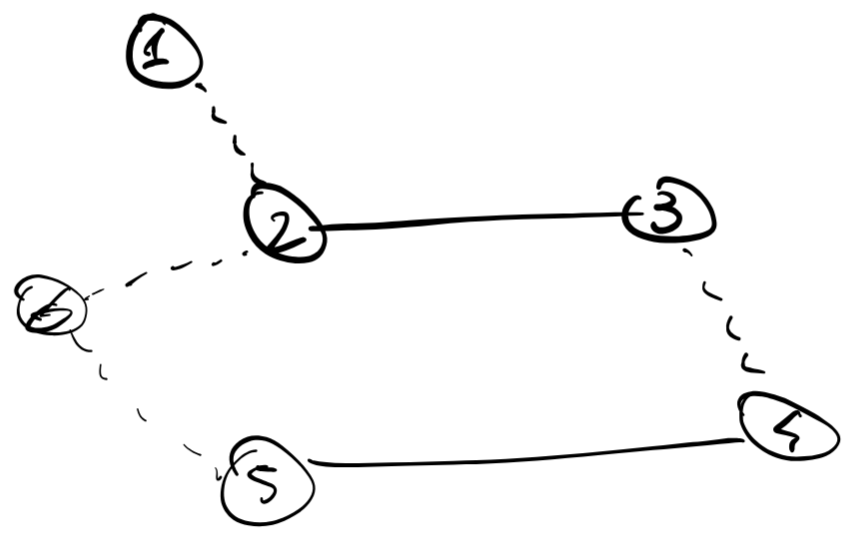
\includegraphics[width=0.8\columnwidth]{img/bipartito1}
	\end{center}
	Partendo da qualsiasi nodo esposto in questo grafo non si possono trovare cammini aumentanti (prova a farci la BFS alternata se non mi credi, stronzo (non ho voglia di scriverla)).\\
	
	\newpage
	
	\section{Tecniche greedy}
	
	\subsection{Problema di LoadBalancing}
	Non ammette una soluzione polinomiale ottima $\in \mathcal{NPO}$.\\
	
	Problema in cui si ha \textbf{un numero di task} di una certa \textbf{durata} e bisogna \textbf{dividerli su varie macchine} in modo da avere la massima \textbf{durata di ogni macchina al minimo possibile}:
	\begin{itemize}
		\item \textbf{Input:} $m > 0$ numero di macchine, $n>0$ numero di task, $(t_i)_{i \in n}$, durate dei task, $t_i > 0$
		
		\item \textbf{Output:} $\alpha: n \rightarrow m$, assegnare ogni task ad una macchina. Il carico della macchina $j$ è definito come 
		$$ L_j := \sum_{i: \alpha (i) = j} t_i$$
		La somma di tutte le durate dei task assegnati a quella macchina. Il carico massimo è
		$$ L := \max_j \{L_j\}$$ 
		il valore più alto di una singola macchina
		
		\item \textbf{Funzione obiettivo:} $L$
		
		\item \textbf{Tipo:} problema di minimizzazione $\min$, devo minimizzare il costo della macchina con il costo più alto
	\end{itemize}
	
	\addcontentsline{toc}{subsubsection}{\protect\numberline{}Teorema}
	\paragraph{Teorema:} LoadBalancing $\in \mathcal{NPO}c$.\\
	
	\textbf{Definizione di $\mathcal{NPO}c$:} un problema di ottimizzazione $\pi$ è $\in \mathcal{NPO}c$ iff $\pi \in \mathcal{NPO}$ e $\hat{\pi} \in \mathcal{NP}c$, il problema di decisione associato è $\mathcal{NP}c$.\\
	
	\newpage
	
	\subsubsection{Algoritmo greedy per LoadBalancing}
	
	Fornisce una \textbf{soluzione approssimata}. Sostanzialmente l'algoritmo consiste nel \textbf{prendere i task} ed associarli sempre alla macchina più "scarica", con la attuale durata complessiva delle task minore.\\
	
	Chiamando $A_i$ l'insieme dei \textbf{task associati alla macchina} $i$.\\
	
	All'inizio sia task associati che carichi totali partono a zero. Si itera su tutti i task, si sceglie la macchina con il carico minore e si aggiunge alla sua lista di task il task $j$ considerato (ed il carico relativo).\\
	Ovviamente è polinomiale: $O(n)$ per cercare tra i task e $O(m)$ per cercare le macchine, quindi il totale $O(nm)$
	
	\begin{algorithm}
		\caption{GreedyLoadBalancing$(n, m)$}
		\begin{algorithmic}
			\STATE $A_i \leftarrow \emptyset$ $\forall i \in n$
			\STATE $L_i \leftarrow \emptyset$ $\forall i \in n$
			\FOR{$j =  0, \, ... \, , m-1$}
				\STATE $\overline{i} \leftarrow \arg \min_i L_i$
				\STATE $A_{\overline{i}} \leftarrow A_{\overline{i}} \cup \{j\}$
				\STATE $L_{\overline{i}} \rightarrow L_{\overline{i}} + t_j$
			\ENDFOR
		\end{algorithmic}
	\end{algorithm}

	\addcontentsline{toc}{subsubsection}{\protect\numberline{}Teorema}
	\paragraph{Teorema:} GreedyBalance è una 2-Approssimazione per Loadbalancing
	
	\begin{proof}
		Chiamando $L^\ast$ il valore della funzione obiettivo della soluzione ottima. \\
		
		\textbf{Osservazione 1:} posso dire che 
		$$ L^\ast \geq \frac{1}{m} \sum_{j} t_j $$
		
		Ovviamente se potessi dividere il totale di tutti i task in modo perfetto su $m$ macchine otterrei una soluzione ideale (1/m del tempo totale per ogni macchina), quindi la soluzione ottima deve essere per forza $\geq$ di questa divisione.\\
		
		\textbf{Osservazione 2 }
		$$ L^\ast \geq \max_j t_j $$
		Il compito più grande qualcuno lo deve fare, quindi il tempo massimo non può essere inferiore al tempo del task più lungo.\\
		
		Sia $\hat{i}$ tale che $L_{\hat{i}} = L$ e sia $\hat{j}$ l'ultimo compito che le è stato assegnato.\\
		
		Prima di assegnare alla macchina $\hat{i}$ l'ultimo carico, questa doveva essere quella con il carico minore di tutte
		$$ L_{\hat{i}} - t_{\hat{j}} \leq L_i ' \;\;\;\;\; \forall i \in m $$
		$$ m (L_{\hat{i}} - t_{\hat{j}}) \leq \sum_i L_i = \sum_j t_j $$
		$$ \implies L_{\hat{i}} - t_{\hat{i}} \leq \frac{1}{m} \sum_j t_j \leq L^\ast $$
		L'ultima parte della disequazione possiamo aggiungerla essendo la stessa cosa della osservazione 1.
		
		$$ L = L_{\hat{i}} = L_{\hat{i}} - t_{\hat{j}} + t_{\hat{j}} \geq 2 \cdot L^\ast $$
		Per la osservazione 2, posso far vedere che $t_{\hat{j}}$ è $\leq L^\ast$, quindi il totale è tutto minore di $2 \cdot L^\ast$. Di conseguenza possiamo evincere il rapporto di approssimazione
		$$ \frac{L}{L^\ast} \leq 2 $$
		
		L'algoritmo quindi è 2-Approssimato.
	\end{proof}
	
	\newpage
	
	% da invertire sopra la frazione, scritto sbagliato
	
	\paragraph{Dimostrazione di tightness:} questa dimostrazione serve a stabilire che $L/L^\ast$ è davvero 2, ovvero che \textbf{il bound non può diminuire ulteriormente} e quel fattore di approssimazione dipende intrinsecamente dall'algoritmo e non da qualche errore nella dimostrazione.\\
	
	\addcontentsline{toc}{subsubsection}{\protect\numberline{}Teorema}
	\paragraph{Teorema:} per ogni $\epsilon > 0$, esiste un input per il problema LoadBalancing tale che GreedyLoadBalancing produce un output con 
	$$ 2 - \epsilon \leq \frac{L}{L^\ast} \leq 2$$
	(ovvero schiaccio quanto voglio il bound).\\
	
	Dobbiamo \textbf{costruire un input} che fa "andare male" l'algoritmo:
	\begin{itemize}
		\item numero di macchine $m > 1/ \epsilon$
		\item numero di task $n = m(m-1)+1$
		\item ci sono $m(m-1)$ task lunghi $1$ e $1$ task lungo $m$, presentati in quest'ordine
	\end{itemize}
	
	I primi $m$ verranno dati ciascuno ad una macchina, e si ripete $m-1$ volte. Alla fine di questi tutte le macchine hanno lo stesso carico.\\
	Poi arriva big task che verrà messo sulla macchina meno carica (sono tutte uguali, quindi una a caso praticamente).\\
	
	Di conseguenza la funzione obiettivo finale sarà:
	$$ L = m - 1 + m = 2m - 1 $$
	
	Non sapendo che alla fine arriva il taskone non possiamo prepararci al suo arrivo. La soluzione ottima sarebbe dare il Titanic ad una macchina e dividere gli altri $m(m-1)$ alle altre macchine; alla fine tutte le macchine avranno lo stesso carico, quindi è sicuramente la soluzione ottima, con valore:
	$$ L = m $$
	
	Il rapporto di prestazione nel primo caso diventa:
	$$ \frac{L}{L^\ast} = \frac{2m-1}{m} = 2 - \frac{1}{m} $$
	
	Essendo un \textbf{algoritmo greedy}, \textbf{l'ordine} dei task è \textbf{importante} ed in questo caso è la differenza tra un input ottimale ed il peggiore.\\
	
	Comunque, magari gli input reali non sono così male, questo algoritmo su input reali potrebbe avere un tasso di approssimazione più basso, potrebbero essere input più favorevoli rispetto alle casistiche considerate in questo modo.\\
	
	\subsubsection{SortedGreedyBalance}
	Sempre sul problema di LoadBalancing, sempre stesso input e output dell'algoritmo precedente.\\
	
	L'algoritmo funziona \textbf{ordinando} in ordine \textbf{decrescente i task} e poi \textbf{chiamando l'algoritmo greedy}:
	
	\begin{algorithm}
		\caption{SortedGreedyBalance$(n, m)$}
		\begin{algorithmic}
			\STATE Sort $t_i$ in Non-increasing order
			\item Run GreedyLoadBalancing$(n,m)$
		\end{algorithmic}
	\end{algorithm}
	
	Ma è davvero meglio? \\
	
	\addcontentsline{toc}{subsubsection}{\protect\numberline{}Teorema}
	\paragraph{Teorema:} SortedGreedyBalance produce una $\frac{3}{2}$-Approssimazione
	
	\begin{proof}
		\textbf{Osservazione 1}: se $n<m$, la soluzione prodotta è ottima (tutti i task a macchine distinte, meglio di così non si può).\\
		
		Da qui in poi viene considerato $n>m$ (almeno una macchina deve avere 2 task assegnati).\\
		
		\textbf{Osservazione 2}: $L^\ast \geq 2 \cdot t_m$. Considerando i task
		$$ t_0 \geq t_1 \geq \, ... \, \geq t_m \geq t_{m+1} \geq \, ... \, \geq t_{n-1} $$
		Almeno una macchina dovrà avere 2 task, uno dai primi $m$ task ed uno dai restanti.\\
		
		\newpage
		
		Sia $\hat{i}$ tale che $L_{\hat{i}} = L$:
		\begin{itemize}
			\item Se $\hat{i}$ ha un task solo, la soluzione è ottima
			\item Se $\hat{i}$ ha più di un compito. Sia $\hat{j}$ l'ultimo compito (ovvero l'indice del task) assegnato a $\hat{i}$
			\item Sicuramente $\hat{j} \geq m$ in quanto i primi $m$ task sono sicuramente dati a macchine distinte (non può esserci una macchina meno carica di una vuota)
		\end{itemize}
		Quindi 
		$$ L = L_{\hat{i}} = \left(L_{\hat{i}} - t_{\hat{j}}\right) + t_{\hat{j}} $$  
		Di conseguenza, sapendo che
		$$ t_{\hat{j}} \leq t_m \leq \frac{1}{2} L^\ast $$
		Possiamo dire
		$$
		\begin{array}{c c}
			\left(L_{\hat{i}} - t_{\hat{j}}\right)  & \leq L^\ast \\
			t_{\hat{j}} & \leq t_{\hat{j}}
		\end{array}
		\implies
		\left(L_{\hat{i}} - t_{\hat{j}}\right) + t_{\hat{j}}  \leq L^\ast + \frac{1}{2} L^\ast = \frac{3}{2} L^\ast
		$$
		In conclusione
		$$ L = L_{\hat{i}} \leq \frac{3}{2}L^\ast $$
		
	\end{proof}
	
	Ci vorrebbe una dimostrazione di tightness, ma questa analisi non è tight, si può dimostrare che l'algoritmo in realtà è una $\frac{4}{3}$-Approssimazione (dimostrazione di \href{https://www.jstor.org/stable/pdf/2099572.pdf}{Graham 1969}).\\
	
	Hochbaum-Shmoys 1988 hanno dimostrato che in realtà LoadBalancing apparitene $\in PTAS$, ovvero si può approssimare con una precisione $\epsilon$ qualunque, e scala esponenzialmente il tempo necessario per l'approssimazione, quindi si sa anche che $\notin FPTAS$.\\
	
	\newpage
	
	\subsection{Problema della selezione dei centri CenterSelection}
	Avendo vari posti dove smistare pacchi e $n$ soldi per costruire un numero limitato di magazzini, bisogna decidere dove piazzarli. Una volta piazzati tutti gli altri centri di smistamento si rivolgono al magazzino più vicino. Si creano delle celle di Varanoi (Check nome) attorno ai magazzini sostanzialmente. Di conseguenza c'è una distanza massima che un centro di smistamento deve coprire per arrivare al magazzino, ovvero un raggio di copertura, tra tutte le soluzioni si vuole minimizzare questo raggio.\\
	
	Hai dei \textbf{punti in uno spazio metrico} e si vogliono \textbf{scegliere} $k$ \textbf{punti} in questo spazio in modo che il \textbf{raggio di copertura} per tutti sia il \textbf{minore possibile}.\\
	
	\paragraph{Spazio metrico:} un'insieme con una funzione distanza $(\Omega, d)$ 
	$$d: \, \Omega  \times \Omega \rightarrow \mathbb{R}^+$$
	
	Con le seguenti proprietà:
	\begin{itemize}
		\item $d(x,y) = d(y,x)$ (simmetria)
		\item $d(x,y) = 0$ iff $x=y$
		\item $d(x,y) \leq d(x,z) + d(z,y)$ (disuguaglianza triangolare)
	\end{itemize}
	L'input per la selezione dei centri sarà immerso in uno spazio metrico.\\
	
	Definizioni: nel mio insieme di punti, qual'è il punto scelto (magazzino) più vicino?
	$$ dist(x,A) := \min_{y \in A} d(x,y) $$
	
	$$ \forall s \in S \;\;\; \delta_c (s) := dist(s,C)$$
	
	$$ \rho_c := \max_{s \in S} \delta_c (s) $$
	
	\newpage
	
	\paragraph{Definizione del problema:} fissiamo uno spazio metrico $(\Omega, d)$
	\begin{itemize}
		\item \textbf{Input:} un \textbf{insieme} $S \subseteq \Omega$ di $n$ \textbf{punti immersi in uno spazio metrico} fissato ed un \textbf{budget} $k>0$
		
		\item \textbf{Soluzione accettabile:} è un \textbf{sottoinsieme} $C \subseteq S$ con $|C| \leq k$ ($\leq k$ punti nello spazio)
		
		\item \textbf{Funzione obiettivo:} $\rho_c$
		
		\item \textbf{Tipo:} $\min$
	\end{itemize}
	Vogliamo minimizzare il massimo dei percorsi.\\
	
	\subsubsection{Algoritmo CenterSelectionPlus} 
	Facciamo finta di avere in input un parametro che non avremo. Stesso input del problema, ma aggiungiamo 
	$$ r \in \mathbb{R}^+ $$
	
	\begin{algorithm}
		\caption{CenterSelectionPlus$(S, k)$}
		\begin{algorithmic}
			\STATE $C \leftarrow \emptyset$
			\WHILE{$S \neq \emptyset$}
				\STATE take any $\overline{s} \in S$
				\STATE $C \leftarrow C \cup \{\overline{s}\}$
				\STATE Remove from $S$ all $s$ t.c. $d(s, \overline{s}) \leq 2r$
			\ENDWHILE
			\IF{$|C| \leq k$}
				\STATE Output $C$
			\ELSE
				\STATE Output "Impossibile"
			\ENDIF
		\end{algorithmic}
	\end{algorithm}
	
	Insieme di centri vuoto, poi finché l'insieme di punto non è vuoto: 
	\begin{itemize}
		\item prende un punto in in $S$
		\item toglie da $S$ tutti i punti con una distanza dal punto preso minore di $2r$
	\end{itemize}
	
	Se la cardinalità di $C$ è $\leq k$ torna $C$, altrimenti dice che è impossibile.\\
	
	\newpage
	
	\addcontentsline{toc}{subsubsection}{\protect\numberline{}Teorema 1}
	\paragraph{Teorema 1:} Se CenterSelectionPlus \textbf{emette un output}, esso è una \textbf{$\frac{2r}{\rho^\ast}$-Approssimazione}.
	
	\begin{proof}
		$\forall s \in S$ con $s$ cancellato da $S$ e sia $\overline{s}$ il centro scelto quando abbiamo cancellato $s$, di conseguenza $d(s, \overline{s}) \leq 2r$:
		$$\rho_c \leq \delta_c (s) \leq d(s, \overline{s}) \leq 2r $$
		Di conseguenza
		$$ \frac{\rho_c}{\rho^\ast} \leq \frac{2r}{\rho^\ast}$$
	\end{proof}
	
	\addcontentsline{toc}{subsubsection}{\protect\numberline{}Teorema 2}
	\paragraph{Teorema 2:} se $r \geq \rho^\ast$, l'algoritmo \textbf{emette un output}.\\
	
	\begin{proof}
		Sia $C^\ast$ una soluzione ottima, una distribuzione di centri che ha come raggio di copertura $\rho^\ast$.  \\
		Sia $\overline{s} \in C$. Chiamiamo $\overline{c}^\ast \in C^\ast$ un centro tale che nella soluzione ottima $\overline{s}$ si rivolge a $\overline{c}^\ast$.\\
		Sia $X$ l'insieme dei punti che nella soluzione ottima $C^\ast$ si rivolgono a $\overline{c}^\ast$
		
		$$ \forall s \in X \;\;\; d(s, \overline{s}) \leq d(s, \overline{c}^\ast) + d(\overline{c}^\ast, \overline{s}) \leq 2 \rho^\ast \leq 2r $$
		
		$\implies$ Quando seleziono $s$, cancello tutti i punti di $X$ (come minimo), perché distano da $s$ meno di $2r$.\\
		$\implies$ Elimino da $S$ un'intera cella di Voronoi di $C^\ast$.\\
		
		$C^\ast$ ha al massimo $k$ celle di Voronoi (avendo $k$ centri al suo interno).\\
		$\implies$ Dopo $\leq k$ passi ho cancellato tutto.\\
	\end{proof}
	%end?
	
	\newpage
	
	Il rapporto di approssimazione abbiamo detto essere $\frac{2r}{\rho^\ast}$, di conseguenza l'insieme delle soluzioni ammissibili è quello dei valori $\geq \rho^\ast$ e la scelta di $r$ \textbf{migliora all'avvicinarsi a} $\rho^\ast$, fino ad essere una 2-Approssimazione con $r = \rho^\ast$.\\
	
	Con $ \frac{1}{2}\rho^asr < r < \rho^\ast$ non è ben definito che output si può ottenere (e se si ottiene un output), ma sicuramente con un $r \leq \frac{1}{2} \rho^\ast$ non si può avere output perché altrimenti porterebbe, secondo l'approssimazione detta sopra, ad un risultato migliore dell'ottimo.\\
	
	Quindi voglio avere un $r$ \textbf{pari a} $\rho^\ast$, ma è un dato che non conosciamo.\\
	
	Al posto di scegliere un punto a caso potrei scegliere punti $\overline{s}$ che sono almeno a distanza $> 2r$ da $C$, facendo terminare l'algoritmo quando non posso sceglierne altri. Equivalente all'algoritmo detto, al posto di cancellare i punti quegli stessi non potranno essere presi in considerazione ma è la stessa cosa.\\
	
	\newpage
	
	\subsubsection{GreedyCenterSelection}
	Stesso input di CenterSelection ma NON abbiamo più il parametro $r$.\\
	
		\begin{algorithm}
		\caption{GreedyCenterSelection$(S, k)$}
		\begin{algorithmic}
			\IF{$|S| \leq k$}
				\STATE output $S$
			\ENDIF
			\STATE choose any $\overline{s} \in S$
			\STATE $C \leftarrow \{ \overline{s}\}$ 
			\WHILE{$|C| \leq k$}
				\STATE select $\overline{s}$ maximizing $d(\overline{s}, C)$
				\STATE $C \leftarrow C \cup \{\overline{s}\}$
			\ENDWHILE
			\STATE Output $C$
		\end{algorithmic}
	\end{algorithm}
	
	
	Se l'insieme dei punti ha cardinalità $\leq k$, torna $S$ (basta prendere tutti i punti). Altrimenti sceglie un qualsiasi $\overline{s} \in S$ e lo sceglie come centro.\\
	
	Finché la cardinalità di $C$ è $<k$ ( quindi sceglierà esattamente $k$ punti) \textbf{sceglie il punto che massimizza la distanza} $d(\overline{s}, C)$ e lo aggiunge a $C$. Alla fine restituisce $C$.\\
	
	%Si comporta in modo simile a quello di prima con $\rho^\ast$, e diventerà una 2-Approssimazione.\\

	% End L4
	
	Cancellare i punti o scegliere il punto più lontano sono equivalenti, non cambia nulla.\\
	
	\newpage
	\addcontentsline{toc}{subsubsection}{\protect\numberline{}Teorema}
	\paragraph{Teorema:} GreedyCenterSelection è una \textbf{2-Approssimazione} per CenterSelection.\\
	
	\begin{proof}
		Supponendo che, per assurdo, l'algoritmo GreedyCenterSelection emetta una soluzione con $\rho>2 \rho^\ast$ (soluzione fuori da $2$ volte il raggio di copertura ottimale). Questo vuol dire che esiste un elemento dell'insieme $S$, $\exists \overline{s} \in S$, con distanza $d (\overline{s}, C) > 2 \rho^\ast$.\\
		
		Sia $\overline{s}_i$ l'$i$-esimo centro aggiunto e sia $\overline{C}_i$ l'insieme dei centri in quel momento. Il punto va scelto in modo che massimizzi la distanza dai centri attuali:
		$$ d(\overline{s}_i, \overline{C}_i) \geq d(\hat{s}_i, C_i) \geq d(\hat{s}, C) > 2 \rho^\ast$$
		Quindi sarà maggiore della distanza di uno dei centri precedenti, che sarà maggiore della distanza finale, a sua volta maggiore di $2 \rho^\ast$.\\
		Alla fine, uno dei punti deve essere distante $>2\rho^\ast$ da tutti i punti scelti.\\
		
		Ma allora l'esecuzione è una delle esecuzioni possibili di CenterSelectionPlus quando $r = \rho^\ast$, ovvero la scelta (prendere quello a distanza massima) è compatibile quella che farebbe l'altro algoritmo (sostanzialmente sta prendendo uno dei punti lontani più di $2r$, non importa quale). GreedyCenterSelection è una particolare esecuzione di CenterSelectionPlus con $r=\rho^\ast$.\\
		
		Ma CenterSelectionPlus con $r= \rho^\ast$ produce un output:\\
		$\implies$ termina entro $k$ iterazioni \\
		$\implies$ tutti gli $s \in S$ sono tali che $d(s,C) \leq 2 \rho^\ast$ \\
		(per i teoremi dimostrati per CenterSelectionPlus).\\
		
		Ma non è vero, dato che: $d(\hat{s}, C) > 2 \rho^\ast$. Assurdo.\\
	\end{proof}
	
	Si potrebbe anche dimostrare che l'algoritmo è tight, ma sappiamo anche che c'è un lower bound per l'approssimazione in tempo polinomiale, quindi possiamo avere una dimostrazione di inapprossimabilità per mostrare che non si può approssimare con un fattore di approssimazione migliore di 2.\\
	
	\newpage
	
	\addcontentsline{toc}{subsubsection}{\protect\numberline{}Teorema}
	\paragraph{Teorema:} Se $\mathcal{P} \neq \mathcal{NP}$ \textbf{non esiste un algoritmo polinomiale} che \textbf{$\alpha$-approssimi} CenterSelection per \textbf{qualche} $\alpha < 2$ (quindi l'algoritmo greedy è polinomialmente ottimo).\\
	
	\begin{proof}
		La dimostrazione si basa su un problema di decisione chiamato DominatingSet: 
		\begin{itemize}
			\item Input: un grafo $G = (V, E)$ ed un $k>0$
			\item Output: $\exists D \subseteq V$, sapere se esiste un insieme di vertici di cardinalità al massimo $k$, $|D| \leq k$, tale che $\forall x \in V$ allora $\exists y \in D$ con $xy \in E$. Sostanzialmente metto sui vertici $k$ guardie ed ogni arco deve essere collegato ad almeno una guardia
		\end{itemize}
		
		Si sa che DominatingSet $\in \mathcal{NP}c$.\\
		
		Dati $G,k$, input di DominatorSet, dobbiamo costruire un'istanza di CenterSelection, quindi innanzitutto uno spazio metrico:
		$$ \Omega = V = S $$
		$$ d (x,y) = 
		\begin{cases}
			0 & \text{ se } \, x=y \\
			1 & \text{ se } \, xy \in E \\
			2 & \text{ se } \, xy \notin E \\
		\end{cases}
		$$
		
		Una cosa non ovvia da dimostrare è la disuguaglianza triangolare, quindi 
		$$ d(x,y) \leq d(x,z) + d(z,y) $$
		Quindi il valore di $ d(x,y)$ può essere solo $1$ o $2$, mentre dall'altro lato della disuguaglianza può valere $2,3$ o $4$. Non devo dirtelo io che $2$ è sempre $\leq 2$.\\
		
		Abbiamo la nostra istanza di CenterSelection$(S,k)$, quindi come input insieme $S$ e budget $k$. \\
		
		Quanto vale il raggio di copertura?
		$$ \rho^\ast (S,k) \in \{1,2\}$$
		Tutte le distanze sono 1 o 2, quindi il raggio sarà 1 o 2.\\
		
		\newpage
		
		Quando succede che la distanza è 1? 
		$$ \rho^\ast (S,k) = 1 $$
		\begin{itemize}[label*=]
			\item \textbf{iff} $\exists C^\ast \subseteq S$, con cardinalità $|C^\ast| \leq k$ e centri tali che $\forall s$, $d(s,C^\ast) \leq 1$ \\
			
			\item \textbf{iff} $\exists C^\ast \subseteq S$ con cardinalità $|C^\ast| \leq k$ tale che $\min_{c \in C^\ast} d(s,c) = 1$.\\
			
			\item \textbf{iff} $\exists C^\ast \subseteq S$ con cardinalità $|C^\ast| \leq k$ tale che $\forall s$,  $\exists c \in C^\ast$ con $sc \in E$.\\
			
			\item \textbf{iff} $C^\ast$ è un dominating set, in quanto è esattamente la definizione di DominatingSet.\\
		\end{itemize}
		
		Un algoritmo $\alpha$-approssimante per CenterSelection fornirà
		$$ \rho^\ast \leq \rho (S,k) \leq \alpha \rho^\ast (s,k) $$
		Ed i casi possibili sono:
		\begin{itemize}
			\item $\rho^\ast = 1$, quindi
			$$ 1 \leq \rho(S,k) \leq \alpha $$
			Se la soluzione ottima è 1 allora mi produce $\alpha$ al limite.\\
			
			\item $\rho^\ast = 2$
			$$ 2 \leq \rho(S,k) \leq 2 \alpha $$
		\end{itemize}
		Sostanzialmente, se potessi risolvere ottimamente CenterSelection in tempo polinomiale, avrei anche una risposta in tempo polinomiale per DominatingSet, dato che, con CenterSelection, se viene 1 la risposta è "sì", mentre se viene 2 la risposta è "no".\\
	\end{proof}
	
	Comunque si parla di un'istanza di CenterSelection abbastanza particolare, quindi questo non significa che non esistano altre versioni ristrette di CenterSelection con migliori fattori di approssimazione. Limitare le istanze solitamente permette di approssimare meglio. Sapere come sono fatti gli input permette di fare meglio.\\
	
	\newpage
	
	\addcontentsline{toc}{subsection}{\protect\numberline{}Funzione Armonica}
	\subsection*{Funzione Armonica}
	Serve per dopo, la lascio qui.\\
	
	Una funzione che \textbf{mappa numeri naturali positivi in reali}:
	$$ H: \mathbb{N}^+ \rightarrow \mathbb{R} $$
	Secondo la funzione:
	$$ H(n) = \sum_{i=1}^n \frac{1}{i} $$
	
	\paragraph{Proprietà 1:}  può essere approssimata per eccesso
	$$ H(n) \leq 1 + \int_1^n \frac{1}{x} dx$$
	$$ \implies H(n) \leq 1 + \ln (n) $$
	
	\paragraph{Proprietà 2:} possiamo dare anche un limite inferiore
	$$ \int_t^{t+1} \frac{1}{x} dx \leq \int_t^{t+1} \frac{1}{t} dx = \frac{1}{t} $$
	
	$$ H(n) = \frac{1}{1} + \frac{1}{2} + \, ... \, + \frac{1}{n} \geq \int_{1}^{2} \frac{1}{x} dx + \int_{2}^{3} \frac{1}{x} dx + \, ... \, + \int_{n}^{n+1} \frac{1}{x} dx =$$
	$$ = \int_1^{n+1} \frac{1}{x} dx = \ln(n+1)$$
	
	Quindi 
	$$ H(n) \geq \ln(n+1) $$
	
	Unendo le due cose:
	$$ \ln (n+1) \leq H(n) \leq 1 + \ln(n) $$
	
	\newpage
	
	\subsection{Problema di SetCover}
	Definizione del problema:
	\begin{itemize}
		\item \textbf{Input:} degli \textbf{insiemi} $S_1, \, ... \, , S_m$ e la loro unione $\bigcup_{i \in m} S_i = U$ (universo), ognuno con dei pesi $w_0, \, ... \, w_{m-1}$
		
		\item \textbf{Soluzioni ammissibili:} scegliere un certo numero di insiemi in modo che siano coperti tutti i punti. $I \subseteq m$ tale che
		$$ \bigcup_{i \in I} S_i = U $$
		
		\item \textbf{Funzione obiettivo:} la somma dei pesi per gli insiemi scelti
		$$ w = \sum_{i \in I} w_i $$
		
		\item \textbf{Tipo:} $\min$, problema di minimizzazione
	\end{itemize}
	
	\subsubsection{GreedySetCover}
	\begin{algorithm}
		\caption{GreedySetCover$()$}
		\begin{algorithmic}
			\STATE $R \leftarrow U$
			\STATE $I \leftarrow \emptyset$
			\WHILE{$R \neq \emptyset$}
				\STATE choose $S_i$ minimizing $\frac{w_i}{|S_i \cap R|}$
				\STATE $I \leftarrow I \cup \{i\}$
				\STATE $R \leftarrow R \setminus S_i$
			\ENDWHILE
			\STATE output $I$
		\end{algorithmic}
	\end{algorithm}
	
	Metto da parte l'insieme universo e prendo un insieme vuoto per i punti. Finché rimangono punti in $R$ scelgo l'insieme che minimizza il rapporto tra costo e punti ancora da coprire presenti in quell'insieme. Una volta scelto, aggiungo l'insieme ed i punti che copre.\\
	Alla fine restituisco $I$.\\
	
	Questo algoritmo è come se assegnasse ad ogni vertice da coprire un costo
	$$\forall s \in S_i \cap R \;\;\;\;\;\;\;\; c(s) := \frac{2_i}{|S_i \cap R|}$$
	
	\newpage
	
	\paragraph{Lemma 1:} Alla fine dell'esecuzione $w = \sum_{s \in U} c(s)$, il \textbf{costo totale è la somma di tutti i costi singoli pagati}.\\
	
	\begin{proof}
		$w = \sum_{i \in I} w_i$, ma il suo costo è ripartito in tutti gli elementi al momento in cui li ho scelti, quindi: 
		$$ w = \sum_{i \in I} w_i = \sum_{i \in I} \sum_{s \in S_i \cap R} c(s) = \sum_{s \in U} c(s) $$
		
		Insomma, la somma dei costi è il costo complessivo, tutto abbastanza ovvio.\\
	\end{proof}
	
	\paragraph{Lemma 2:} per ogni $k$ 
	$$ \sum_{s \in S_k} c(s) \leq H(|S_k|) w_k $$
	Se sommiamo i costi attributi all'interno di ogni insieme, quello che si ottiene è minore uguale della funzione armonica calcolata nel punto pari alla cardinalità dell'insieme $S_k$, moltiplicato per il peso $w_k$. Sì insomma, si capisce meglio dalla disequazione.\\
	
	\begin{proof}
		Prendendo $S_k=\{s_1, \, ... \, , s_d\}$, con i vertici enumerati in ordine di copertura (mettendo per primi i vertici che sono stati coperti per primi, quindi a blocchi di elementi, un "blocco" per ogni volta che viene scelto un'insieme).\\
		
		Consideriamo l'iterazione che copre $s_j$ e di conseguenza il momento prima che $s_j$ venga coperto tutti i vertici dopo sicuramente non sono coperti
		$$ \{s_j , s_{j+1}, \, ... \, , s_d\} \subseteq R $$
		$$ \implies |S_k \cap R| \geq d - j + 1 $$
		
		\newpage
		
		Per la definizione di costo sappiamo che al passo $h$ prima che venga scelto il vertice $s_j$:
		$$ \implies c(s_j)  =\frac{w_h}{|S_h \cap R|} \leq \frac{w_k}{|S_k \cap R|} \leq \frac{w_k}{d-j+1}$$
		Ed il costo è sempre minore di quelli successivi essendo che l'algoritmo cerca di minimizzarlo.\\
		
		Di conseguenza:
		$$ \sum_{s \in S_k} c(s) \leq \sum_{j=1}^d c(s_j)  \leq \sum_{j=1}^d \frac{w_k}{d-j+1} =$$
		$$ = \frac{w_k}{d} + \frac{w_k}{d-1} + \, ... \, + \frac{w_k}{1} = w_k \left(\frac{1}{1} + \frac{1}{2} + \, ... \, + \frac{1}{d} \right) = $$
		$$ = w_k H(d) = w_k H(|S_k|) $$ 
	\end{proof}

	%End L5
	
	\newpage
	
	Dai due lemmi segue il teorema.
	
	\addcontentsline{toc}{subsubsection}{\protect\numberline{}Teorema}
	\paragraph{Teorema:} Sia $M = \max_i |S_i|$ (massima cardinalità di un insieme). Allora GreedySetCover è \textbf{una $H(M)$-approssimazione} per SetCover (l'\textbf{approssimazione è in funzione dell'input}, al crescere di quest'ultimo cresce il fattore di approssimazione). \\
	
	\begin{proof}
		Sia $I^\ast$ una soluzione ottima (come insieme di indici) e di conseguenza 
		$$ w^\ast = \sum_{i \in I^\ast} w_i $$
		Sarà il minimo possibile.\\
		
		Per il Lemma 2 
		$$ w_i \geq \frac{\sum_{s \in S_i} c(s)}{H(|S_i|)} \geq \frac{\sum_{s \in S_i} c(s)}{H(M)} \implies $$
		$H$ è una funzione monotona, quindi con un valore maggiore risultato maggiore, di conseguenza al denominatore diventa più piccolo.\\
		
		Quindi 
		$$ \implies w^\ast = \sum_{i \in I^\ast} w_i = \sum_{i \in I^\ast} \sum_{s \in S_i} c(s) $$
		
		%TODO Check formule
		
		La somma dei pesi degli insiemi è pari alla somma del costo di tutti gli elementi di tutti gli insiemi. In questa sommatoria stiamo sommando tutti gli elementi dell'universo, quindi (per il Lemma 1)
		$$ \geq \sum_{s \in U} c(s) = w $$
		
		Ed inoltre possiamo vedere che, applicando, in ordine, la prima e seconda uguaglianza vista sopra
		$$ w^\ast = \sum_{i \in I^\ast} w_i \geq \sum_{i \in I^\ast} \frac{\sum_{s \in S_i} c(s)}{H(M)} \geq \frac{w}{H(M)} $$
		$$ \implies \frac{w}{w^\ast} \leq H(M)$$
	\end{proof}
	
	\paragraph{Osservazione:} $M$ è sicuramente minore della dimensione dell'input, \\ $M \leq |U| = n$, quindi $H(M) \leq H(n) = O(\log n)$.\\
	
	\paragraph{Corollario:} GreedySetCover è \textbf{una $O(\log n)$-approssimazione}. L'approssimazione peggiora con $O(\log n)$. Non eccezionale come cosa ma ci accontentiamo.\\
	
	\addcontentsline{toc}{subsubsection}{\protect\numberline{}Tightness}
	\paragraph{Tightness:} dobbiamo costruire un \textbf{input} su cui l'algoritmo va abbastanza male da \textbf{verificare} il nostro \textbf{upper bound} per l'approssimazione.\\
	
	L'input (universo) di dimensione $n$ è composto da due insiemi di costo $1 + \epsilon$, ognuno con al suo interno $n/2$ punti. \\
	Poi ci sono altri insiemi, tutti di costo 1:
	\begin{itemize}
		\item uno che contiene $n/4$ elementi da ognuno dei due insiemi iniziali (cardinalità totale $n/2$)
		\item uno che contiene $n/8$ elementi da ognuno dei due insiemi iniziali (cardinalità totale $n/4$)
		\item Puoi indovinare come continua
	\end{itemize}
	Esempio:
	
	\begin{center}
		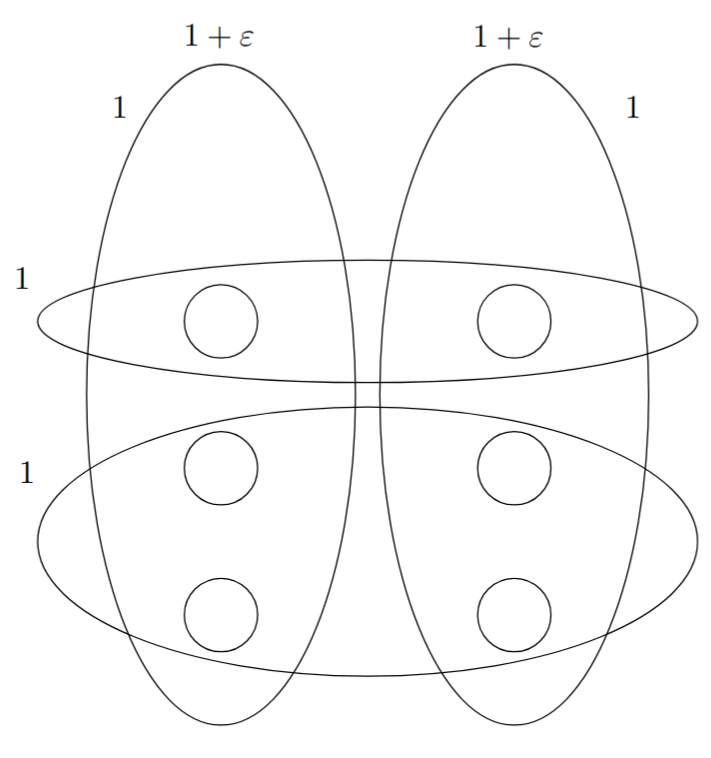
\includegraphics[width=0.5\columnwidth]{img/VertexCoverInput}
	\end{center}
	
	La soluzione ottima ovviamente è prendere i due insiemi più grandi per un costo di $2(1 + \epsilon)$.\\
	
	\newpage
	
	Ma GreedySetCover su questo input sceglierà per primo l'insieme che copre $n/2$ punti con costo $1$ in quanto 
	$$ \frac{1}{n/2} < \frac{1+\epsilon}{n/2} $$
	
	Al passaggio dopo i due insiemi grossi conterranno $n/4$ nuovi elementi e si ripeterà:
	$$ \frac{1}{n/4} < \frac{1+\epsilon}{n/4} $$
	
	Quindi non sceglierà mai i due insiemi grandi ma sempre le intersezioni che coprono sempre meno elementi. Di conseguenza:
	$$ w = \log n $$
	$$ w^\ast = 2 + 2 \epsilon$$
	$$ \implies \frac{w}{w^\ast} = \frac{\log n}{2 + 2 \epsilon} = \Omega (\log n)$$
	
	Quindi questo algoritmo fa le scelte peggiori possibili, ed è l'input peggiore possibile.\\
	
	\paragraph{Fun fact:} Se $P \neq NP$ non esiste un algoritmo che approssimi SetCover meglio di $(1 - O(1)) \log n$. Questo pone SetCover nell'insieme dei problemi $\log n$-APX.\\
	
	\newpage
	
	\section{Tecnica di Pricing}
	
	\subsection{Problema VertexCover}
	
	Definizione del problema: 
	\begin{itemize}
		\item \textbf{Input:} un grafo non orientato $G =(V,E)$ con dei pesi/costi per ogni nodo $w_i \in \mathbb{R}^+$, $i \in V$
		\item \textbf{Soluzione ammissibile:} $X \subseteq V$ tale che $\forall e \in E$, $e \cap X \neq \emptyset$, ogni lato deve avere una delle due estremità dentro la soluzione
		\item \textbf{Funzione obiettivo:} somma dei pesi $\sum_{i \in X} w_i$
		\item \textbf{Tipo:} minimizzazione $\min$
	\end{itemize}
	
	\paragraph{Pricing-based Solution:} I problemi basati sul pricing funzionano basandosi sull'idea che ogni lato offre una cifra per farsi coprire, ed i vertici devono decidere cosa fare, ovvero se entrare nella soluzione o meno, ottenendo la cifra di tutti i lati che copre. I vertici sono una gang che vuole massimizzare il costo dei lati. Ad ogni lato si associa un prezzo per "farsi coprire".\\
	Quindi si ha un \textbf{pricing} $(P_e)_{e \in E}$ \textbf{per ogni lato}.\\
	
	Un pricing $(P_e)_{e \in E}$ è \textbf{equo} se \textbf{iff} $\forall i$
	$$ \sum_{e \in E, i \in e} P_e \leq w_i $$
	Ovvero, i \textbf{lati}, in totale, \textbf{non offriranno più} di quanto "richiede" il vertice, ovvero \textbf{del costo del vertice}. Zero su tutti i lati soddisfa banalmente questa proprietà. Verranno considerati solo di pricing equi.\\
	
	\newpage
	
	\paragraph{Lemma 1:} Se $(P_e)_{e \in E}$ è un \textbf{pricing equo} allora se \textbf{sommo tutti i prezzi} di tutti i lati \textbf{ottengo} un \textbf{valore minore uguale} della \textbf{soluzione ottima}
	$$ \sum_{e \in E} P_e \leq w^\ast $$
	
	\begin{proof}
		Considerando $X^\ast \subseteq V$ soluzione ottima e il peso relativo
		$$ w^\ast = \sum_{i \in X^\ast} w_i $$
		
		Per la definizione di equità: $\forall i$ 
		$$ w_i \geq \sum_{e \in E, i \in e} P_e $$
		il peso di ogni nodo è maggiore della somma dei costi dei lati su di esso.\\
		
		Quindi 
		$$ w^\ast = \sum_{i \in X^\ast} w_i \geq \sum_{i \in X^\ast} \sum_{e \in E, i \in e} P_e \geq \sum_{e \in E} P_e $$
		La soluzione ottima è per forza maggiore della somma di tutti i lati, quindi maggiore della somma del prezzo di tutti i lati (per ammissibilità).\\
	\end{proof}
	
	Sostanzialmente,  se il pricing è equo il costo del nodo deve essere $\geq$ della somma dei pricing dei suoi lati, quindi la soluzione ottima, in quanto composta dal peso dei nodi, non potrà essere minore della somma totale dei pricing.\\
	
	\paragraph{Pricing stretto:} Il pricing $(P_e)_{e \in E}$ è \textbf{stretto} su $\hat{i}$ (un vertice specifico) iff
	$$ \sum_{e \in E, \hat{i} \in e} P_e < w_{\hat{i}} $$
	In breve, "\textbf{pricing stretto}" vuol dire che \textbf{non soddisfa quanto chiede il vertice}, somma dei pricing di quel vertice minore del costo del vertice.\\
	
	\newpage
	
	\subsubsection{PricingVertexCover}
	L'input e sempre $G = (V,E)$, $w_i \in \mathbb{R}^+$, $i \in V$.
	
	\begin{algorithm}
		\caption{PricingVertexCover}
		\begin{algorithmic}
			\STATE $P_e \leftarrow 0$, $\forall e \in E$
			\WHILE{$\exists \hat{e} = \{\hat{i}, \hat{j}\}$ t.c. $(P_e)$ è stretto su $\hat{i}$ e $\hat{j}$}
				\STATE Sia $\hat{e} = \{\hat{i}, \hat{j}\}$ quello che minimizza 
				$$\Delta \leftarrow \min \left(w_{\hat{i}} - \sum_{e \in E, \hat{i} \in e} P_e, w_{\hat{i}} - \sum_{e \in E, \hat{j} \in e} P_e \right)$$
				\STATE $P_{\hat{e}} \leftarrow P_{\hat{e} + \Delta}$
			\ENDWHILE
		\end{algorithmic}
	\end{algorithm}
	
	Inizialmente attribuisce a tutti i lati un prezzo 0.\\
	
	Finché \textbf{esiste un lato} tale che $(P_e)$ è stretto su $\hat{i}$ e su $\hat{j}$, $\exists \hat{e} = \{\hat{i}, \hat{j}\}$, ovvero il \textbf{pricing è stretto su entrambe le estremità}, quindi per entrambi il costo del vertice è maggiore della somma dei pricing offerti, finché vale questa condizione si \textbf{viene scelto il lato} $\hat{e} = \{\hat{i}, \hat{j}\}$ tale che \textbf{minimizza} di quanto dovrebbe \textbf{aumentare la sua offerta} per \textbf{rendere non stretto} il costo di uno dei vertici adiacenti.\\
	
	Alla fine \textbf{restituisce l'insieme dei vertici} $i$ tali per cui $P_e$ \textbf{su} $i$ \textbf{non è stretto}.\\
	
	Partono tutti a zero, guardo vertice per vertice quanto stanno ricevendo dai lati adiacenti, ed all'inizio ovviamente non sarà stretto su nessun vertice.\\
	Quanto dovrebbe offrire in più ogni lato per rendere stretto il pricing su uno dei due vertici a cui è collegato? Calcolo il valore per tutti e prendo il minimo.\\
	Ripeto sui lati non ancora stretti per entrambe le estremità, finché sono presenti lati con questa caratteristica.\\
	
	Alla fine restituisce i vertici "contenti", quindi i vertici che prendono quanto chiedono, ovvero i vertici con pricing non stretto.
	
	%End L6

	\newpage
	
	Ricordando il lemma sul pricing equo.
	
	\paragraph{Lemma:} alla fine di PricingVertexCover il costo $w \leq 2 \sum_{e \in E} P_e$ è minore uguale al doppio della somma dei prezzi. \\
	
	\begin{proof}
		$$ w = \sum_{i \in output} w_i = \sum_{i: P_e \text{ non stretto su } i} w_i = $$
		Emettiamo in output i vertici tali per cui il pricing su quel vertice non è stretto. Per la definizione di "stretto", possiamo continuare dicendo che: 
		$$ = \sum_{i \in output} \sum_{e \in E, i \in e} P_e$$
		Qua stiamo sommando per tutti i vertici nell'output i prezzi di alcuni lati, ma \textbf{ognuno dei lati può comparire al massimo due volte}, se entrambe le estremità di quel lato stanno nell'output. Quindi:
		$$ \sum_{i \in output} \sum_{e \in E, i \in e} P_e \leq 2 \sum_{e \in E} P_e$$
	\end{proof}
	
	\addcontentsline{toc}{subsubsection}{\protect\numberline{}Teorema}
	\paragraph{Teorema:} PricingVertexCover è una 2-Approssimazione.\\
	
	\begin{proof}
		$$ \frac{w}{w^\ast} \leq \frac{2 \sum_{e \in E} P_e}{w^\ast} \leq \frac{2 \sum_{e \in E} P_e}{\sum_{e \in E} P_e} = 2$$
		Per il Lemma 2, $w$ è minore di 2 volte la somma totale dei prezzi, mentre la soluzione ottima $w^\ast$ è per forza maggiore della somma totale dei prezzi. \\
	\end{proof}
	
	Non si sa se esiste un'approssimazione migliore, non si conosce una $\gamma$-approssimazione con $\gamma < 2$. Si sa che non esiste un PTAS, quindi c'è per forza un minimo di approssimazione ma non si sa per certo quale sia.\\
	
	\newpage
	
	\subsection{Problema DisjointPaths}
	
	Problema dei \textbf{cammini disgiunti}. L'idea è, su un grafo orientato, ci sono $k$ \textbf{sorgenti} ed altrettante \textbf{destinazioni}, una lista di sorgenti e destinazioni. Vogliamo \textbf{collegare il maggior numero di sorgenti e destinazioni tramite un cammino}, con il vincolo di non usare ogni lato più di una volta. Verrà considerata una versione con un parametro $c$ che determina la congestione, ovvero \textbf{ogni lato non può essere usato più di $c$ volte}.\\
	
	Definizione: 
	\begin{itemize}
		\item \textbf{Input:} un grafo orientato $G = (N,A)$, la lista delle sorgenti $s_0, \, ... \, , s_k \in N$, la lista delle destinazioni $t_0, \, ... \, , t_k \in N$ ed un parametro $c \in \mathbb{N}^+$
		\item \textbf{Output:} $I \subseteq k$ e $\forall i \in I$ un cammino $\pi_i: s_i \rightarrow t_i$ tale che nessun arco di $G$ sia usato da più di $c$ cammini
		\item \textbf{Funzione obiettivo:} la cardinalità $|I|$, ovvero il numero di cammini trovati
		\item Tipo: massimizzazione, $\max$
	\end{itemize}
	
	Da notare che con i grafi orientati si parla di nodi (da qui $N$), non vertici, e archi (da qui $A$), non lati.\\
	
	Per l'esecuzione dell'algoritmo \textbf{assoceremo} ad \textbf{ogni arco} un \textbf{funzione lunghezza}:
	$$ \ell: \, A \rightarrow \mathbb{R}^+ $$
	
	Che può \textbf{variare nel tempo}, quindi va \textbf{specificato il momento} in cui viene considerata. Di conseguenza si avrà una lunghezza dei cammini: con $\pi = <x_1, \, ... \, , x_i>$
	$$ \ell (\pi) = \ell (x_1, x_2) + \ell (x_2, x_3) + \, ...  \, + \ell (x_{i-1}, x_i) $$
	
	\newpage
	
	\subsubsection{GreedyPaths}
	Input come sopra, grafo, sorgenti, destinazioni, capacità. Si aggiunge un parametro $\beta>1$.
	
	\begin{algorithm}
		\caption{GreedyPaths}
		\begin{algorithmic}
			\STATE $I \leftarrow \emptyset$
			\STATE $P \leftarrow \emptyset$
			\STATE $\ell(a) = 1 $, $\forall a \in A$
			\WHILE{$true$}
				\STATE find shortest path $\pi_i: \, s_i \rightarrow t_i$ with $i \notin I$
				\IF{such path does not exist}
					\STATE break
				\ENDIF
				\STATE $I \leftarrow I \cup \{i\}$
				\STATE $P \leftarrow P \cup \{\pi_i\}$
				\FORALL{$a \in \pi_i$}
					\STATE $\ell (a) \leftarrow \ell (a) \cdot \beta$
					\IF{$\ell(a) = \beta^c$}
						\STATE remove $a$
					\ENDIF
				\ENDFOR
			\ENDWHILE
			\STATE Output $I$, $P$
		\end{algorithmic}
	\end{algorithm}
	
	L'insieme $I$ è l'insieme delle \textbf{coppie già collegate}, all'inizio vuoto, così come l'insieme di \textbf{cammini} $P$. La funzione \textbf{lunghezza all'inizio vale 1 per tutti} gli archi. Poi si ha un ciclo infinito in cui: 
	\begin{itemize}
		\item trova il \textbf{percorso più breve} (secondo la lunghezza $\ell$) \textbf{tra} una \textbf{coppia sorgente e destinazione non ancora collegata}
		\item \textbf{se} tale percorso \textbf{non esiste} per nessuna delle coppie rimaste, \textbf{esce} dal ciclo
		\item se ho trovato un percorso, \textbf{aggiungo} la coppia di \textbf{nodi collegati ad} $I$ ed il relativo path in $P$
		\item per tutti gli archi nel cammino, \textbf{moltiplico} il \textbf{lunghezza per} $\beta$, rendendoli più costosi e meno appetibili per i prossimi path. Inoltre se un \textbf{arco è stato usato} $c$ volte \textbf{viene rimosso}
	\end{itemize}
	Alla fine \textbf{restituisce l'insieme delle coppie collegate ed i relativi path}.\\
	
	\newpage
	
	Quando si dice "trovare il cammino minimo", bisogna usare più iterazioni di Dijkstra per trovarli tutti.\\
	
	\paragraph{Definizione:} In un certo istante dell'esecuzione un \textbf{cammino} $\pi$ è definito \textbf{corto} iff la sua \textbf{lunghezza} è \textbf{minore di} $\beta^c$, quindi $\ell(\pi) < \beta^c$. \\
	
	\paragraph{Definizione:} In un certo istante, un \textbf{cammino} $\pi$ è \textbf{utile} se \textbf{collega una coppia nuova} $i \notin I$. L'algoritmo considera solo cammini utili ed il più corto tra quelli esistenti.\\
	
	L'algoritmo avrà più \textbf{fasi}, una in cui seleziona solo cammini corti utili, poi una in in cui sceglie cammini lunghi utili, e termina quando sono finiti tutti i cammini utili.\\
	
	Considerando il programma nella fase in cui sono \textbf{finiti cammini corti utili}, chiameremo $\overline{\ell}, \overline{I}, \overline{P}$ rispettivamente lunghezza, insieme di coppie collegate ed i relativi path in quel momento, ovvero subito dopo che è stato aggiunto l'ultimo cammino utile.\\
	Alla fine dell'esecuzione chiameremo i parametri $\ell_{out}, I_{out}, P_{out}$.\\
	
	\paragraph{Lemma 1:} Sia $i \in I^\ast \setminus I_{out}$, una coppia \textbf{collegata dalla soluzione ottima ma non dalla soluzione dell'algoritmo}, allora 
	$$\overline{\ell} (\pi_i^\ast) \geq \beta^c$$
	Ovvero il costo del path è superiore a $\beta^c$. \\
	%TODO Check la frase: (Immaginando che non vengano rimossi, per la prima fase dell'esecuzione non cambia niente, sono cammini troppo costosi per essere considerati).\\
	
	\begin{proof}
		$i \in I^\ast \setminus I_{out}$, se fosse vera la condizione $\overline{\ell} (\pi_i^\ast) < \beta^c$ selezioneremmo quel path, ma noi stiamo guardando il momento in cui non sono più presenti cammini corti, quindi non è possibile.\\
		Quindi se $\overline{\ell} (\pi_i^\ast) < \beta^c$ per costruzione dell'algoritmo verrebbe incluso, ma il presupposto è esattamente il contrario.\\
	\end{proof}
	
	\newpage
	
	\paragraph{Lemma 2:} se \textbf{sommo la lunghezza di tutti gli archi} ottengo:
	$$ \sum_{a \in A} \overline{\ell}(a) \leq \beta^{c+1} |\overline{I}| + m $$
	La somma della lunghezza è minore uguale di $\beta^{c+1}$ per il numero di cammini corti $+ m$, con $m$ il numero totale di archi.\\
	
	\begin{proof}
		Per induzione. All'inizio: 
		$$ \sum_{a \in A} \ell (a) = m  \leq \beta^{c+1} |\overline{I}| + m$$
		Supponendo che 
		$$ \ell_1 \xrightarrow[i, \pi_i]{} \ell_2 \rightarrow \, ... \, \rightarrow \overline{\ell}$$
		
		Quindi nel momento di transizione tra $\ell_1$ e $\ell_2$ vengono aggiunti $i$ e $\pi_i$. \\
		Possiamo vedere che $\ell_2$ diventa:
		$$
		\ell_2 (a) = \begin{cases}
			\ell_1 (a) & a \notin \pi_i \\
			\ell_1 (a) \cdot \beta \;\; & a \in \pi_i \\
		\end{cases}
		$$
		
		Quindi domandandoci di quanto sia aumentata la lunghezza degli archi possiamo vedere che:
		$$ \sum_{a \in A} \ell_2 (a) - \sum_{a \in A} \ell_1 (a) = $$
		
		Ma possiamo considerare solo gli archi nel path $\pi$ in quanto l'aumento per gli altri è 0: 
		$$ = \sum_{a \in \pi} \left(\ell_2 (a) - \ell_1 (a)\right) =$$
		
		Ma per passare da $\ell_1$ a $\ell_2$ abbiamo moltiplicato $\ell_1$ per $\beta$, quindi
		$$ = \sum_{a \in \pi} \left( \beta \ell_1 (a) - \ell_1 (a) \right) = $$
		
		Quindi possiamo raccogliere e dire che, per definizione di tutti i path scelti negli istanti precedenti $\overline{\ell}$
		$$ = (\beta -1) \sum_{a \in A} \ell_1 (a) = (\beta -1) \ell_1 (\pi) < (\beta -1) \beta^c \leq \beta^{c+1} $$
	
		Ad ognuno dei $|\overline{I}|$ passi (quindi per ognuno dei cammini trovati) possiamo dire che aumento la somma di al più $\beta^{c+1}$. Si aggiunge $m$ in quanto valore iniziale di tutti gli archi, ovviamente presente.\\
	\end{proof}
	
	\paragraph{Osservazione 1:} Tutti i \textbf{cammini} nella \textbf{soluzione ottima} ma \textbf{non in quella dell'algoritmo} sono \textbf{maggiori di}
	$$ \sum_{i \in I^\ast \setminus I_{out}} \overline{\ell} (\pi_i^\ast) \geq \beta^c |I^\ast \setminus I_{out}|$$
	Per il Lemma 1.\\
	
	\paragraph{Osservazione 2:} Nella \textbf{soluzione ottima nessun arco} è \textbf{usato più di $c$ volte}, comunque è vincolata, quindi
	$$ \sum_{i \in I^\ast \setminus I_{out}} \overline{\ell}(\pi_i^\ast) \leq c \sum_{a \in A} \overline{\ell} (a) \leq $$

	e per il lemma 2 
	$$ \leq c \left( \beta^{c+1}|\overline{I}| + m \right) $$
	
	\nn 
	Quindi, \textbf{usando le osservazioni}: 
	$$ \beta^c |I^\ast| \leq \beta^c |I^\ast \setminus I_{out}| + \beta^c |I^\ast \cap I_{out}| \leq $$
	
	La prima parte, per l'osservazione 1, è maggiorata da
	$$ \leq \sum_{i \in I^\ast \setminus I_{out}} \overline{\ell} (\pi_i^\ast) + \beta^c |I_{out}| \leq $$
	
	Ma questo corrisponde all'osservazione 2:
	$$ \leq c \left( \beta^{c+1}|\overline{I}| + m \right) + \beta^c |I_{out}| \leq  c \left( \beta^{c+1}|I_{out}| + m \right) + \beta^c |I_{out}| $$
	
	Dividendo per $\beta^c$:
	$$ |I^\ast| \leq c \cdot \beta \cdot |I_{out}| + \frac{cm}{\beta^c} + |I_{out}| \leq $$
	
	Aggiungendo un $|I_{out}|$ sicuramente il valore rimane maggiore, lo aggiungiamo per raccogliere:
	$$ \leq c \cdot \beta \cdot |I_{out}| + \frac{cm}{\beta^c} |I_{out}| + |I_{out}| = |I_{out}| \left(c \beta + \frac{cm}{\beta^c} + 1\right) $$
	
	Quindi
	$$ \frac{|I^\ast|}{|I_{out}|} \leq c \left(\beta + m \beta^{-c}\right) + 1$$
	
	Ma bisogna trovare un $\beta$ adeguato, e considereremo
	$$ \beta = m^{\frac{1}{c+1}}$$
	
	Con questa scelta il rapporto visto può essere maggiorato da:  
	$$ \frac{|I^\ast|}{|I_{out}|} \leq c \left(m^{\frac{1}{c+1}} + m^{1-\frac{1}{c+1}}\right) + 1 = 2c m^{\frac{1}{c+1}} + 1 $$
	
	\addcontentsline{toc}{subsubsection}{\protect\numberline{}Teorema}
	\paragraph{Teorema:} GreedyPath fornisce una \textbf{$\left(2c \cdot m^{\frac{1}{c+1}} + 1\right)$-approssimazione} per Disjoint paths.
	
	\vfill
	
	Esempio di valori:
	\begin{center}
		$$
		\begin{array}{c | c}
			c & \\
			\hline
			1 & 2 \sqrt{m} + 1 \\
			2 & 4 \sqrt[3]{m} + 1 \\
			3 & 6 \sqrt[4]{m} + 1 \\
		\end{array}
		$$
	\end{center}
	
	Dipende da $c$ e dal numero di archi $m$. Si ha $c$ che determina un parametro lineare ed una radice che riduce il valore di $m$. Cresce al numero di archi, ma decresce con $c$.\\
	
	%End L7 
	
	L'approssimazione migliora nel caso di coppie ripetute.\\
	
	\newpage
	
	\section{Tecniche basate sull'arrotondamento}
	\addcontentsline{toc}{subsection}{\protect\numberline{}Programmazione Lineare}
	\subsection*{Programmazione Lineare}
	
	Serve per il prossimo algoritmo, bear with me.\\
	
	La programmazione lineare ($LP$) può essere \textbf{descritta come problema di ottimizzazione}: 
	\begin{itemize}
		\item \textbf{Input:} una \textbf{matrice di razionali} $A \in \mathbb{Q}^{m \times m}$, un \textbf{vettore} $b \in \mathbb{Q}^m$, \textbf{vettore} $c \in \mathbb{Q}^n$
		
		\item \textbf{Soluzioni ammissibili:} tutti i \textbf{vettori} $x \in \mathbb{Q}^n$ \textbf{tali che} $Ax \geq b$
		
		\item \textbf{Funzione obiettivo:} $c^T x$
		
		\item \textbf{Tipo:} minimizzazione $\min$
	\end{itemize}
	
	Si sa che $LP \in \mathcal{PO}$ (il più famoso è algoritmo di Karmarkar).\\
	
	\addcontentsline{toc}{subsubsection}{\protect\numberline{}PL Intera}
	\subsection*{PL Intera}
	Programmazione lineare intera ($ILP$):
	\begin{itemize}
		\item \textbf{Input:} matrice $A \in \mathbb{Q}^{m \times m}$, $b \in \mathbb{Q}^m$,  $c \in \mathbb{Q}^n$
		
		\item \textbf{Soluzioni ammissibili:} tutti i vettori $x \in \mathbb{Z}^n$ tali che $Ax \geq b$
		
		\item \textbf{Funzione obiettivo:} $c^T x$
		
		\item \textbf{Tipo:} minimizzazione $\min$
	\end{itemize}
	
	Cercando una\textbf{ soluzione intera al posto che razionale} il problema diventa $ILP \in \mathcal{NPO}c$.\\
	
	\newpage
	
	\subsection{VertexCover via Rounding}
	Soluzione per VertexCover \textbf{basata sull'arrotondamento}.\\
	
	\paragraph{Programmazione lineare per VertexCover:} Per il problema VertexCover $\pi$: Input: $G = (V,E)$, con pesi $w_i \in \mathbb{Q}^+$, $\forall i \in V$ (già definito prima, non riscritto). \\
	
	Il problema di programmazione lineare intera associato a $\pi$ diventa $ILP(\pi)$: $x \in \mathbb{Z}^n$, ed i vincoli sono: 
	$$
	\begin{cases}
		x_i + x_j \geq 1 & \forall \{i,j\} \in E \\
		x_i \geq 0 & \forall i \in V \\
		x_i \leq 1 & \forall i \in V
	\end{cases}
	$$
	La funzione \textbf{obiettivo da minimizzare} è:
	$$ \sum_{i \in V} w_i x_i $$
	
	I vincoli sostanzialmente dicono che il nodo è o 0 o 1, possono essere solo numeri interi, quindi il nodo è preso oppure no, ed il vincolo $\geq 1$ stabilisce che ogni arco è preso da almeno un nodo. \\
	Ma questo rimane un problema $ \in \mathcal{NPO}c$.\\
	
	La versione "rilassata" di $\pi$ è uguale ma \textbf{risolto con} $x \in \mathbb{Q}^n$ ($LP$ non $ILP$). Stessi vincoli, stessa funzione obiettivo.\\
	
	Quindi, partiamo dal \textbf{problema di VertexCover} $\pi$, lo abbiamo trasformato in un problema di \textbf{programmazione lineare intera} $ILP(\pi)$, ci dimentichiamo della parte intera , \textbf{diventa} $LP(\pi)$, ed \textbf{arrotondiamo} a partire dalla soluzione ottima $x^\ast$ di $LP(\pi)$: 
	$$ \pi = (V,E), w_i  \xrightarrow[]{} 
	\begin{array}{c}
		ILP(\pi) \\
		w^\ast_{ILP} \\
	\end{array}
	\xrightarrow[]{}
	\begin{array}{c}
		LP(\pi) \\
		w^\ast_{LP}
	\end{array}
	\xrightarrow{x^\ast}
	\text{ Rounding }
	\xrightarrow{}
	\hat{x}
	$$
	$$ 
	\hat{x} = \begin{cases}
		0 & \text{ se } x^\ast_i <  \frac{1}{2} \\ 
		1 & \text{ se } x^\ast_i \geq  \frac{1}{2} 
	\end{cases}
	$$
	
	Chiamando $w^\ast_{ILP}$ la funzione obiettivo di $ILP(\pi)$ e $w^\ast_{LP}$ la funzione obiettivo di $LP(\pi)$.\\
	
	\paragraph{Lemma 1:} $w^\ast_{LP} \leq w^\ast_{ILP}$.\\
	
	\begin{proof}
		Il problema rilassato ha un superinsieme di soluzioni ammissibili, quindi la soluzione ottima sicuramente non può peggiorare, può solo essere migliore.\\
	\end{proof}
	
	\paragraph{Lemma 2:} $\hat{x}$ è una \textbf{soluzione ammissibile} di $ILP(\pi)$.\\
	
	\begin{proof}
		Ricordando i vincoli
		$$\begin{cases}
			\hat{x}_i + \hat{x}_j \leq 1 & \forall \{i,j\} \in E \\
			0 \leq \hat{x}_i \leq 1 & \forall i \in V
		\end{cases}
		$$
		E la definizione di $\hat{x}_i$ (sopra).\\
		
		Inoltre sappiamo che $x^\ast_i$ rispetterà, in quanto soluzione ammissibile, gli stessi vincoli che sono presenti per $\hat{x}$.\\
		
		L'unico vincolo importante da verificare è che la somma sia $\geq 1$ e l'unico caso in cui può non succedere è quando entrambi sono $=0$ 
		$$ \hat{x}_i + \hat{x}_j \ngeq 1 \implies \hat{x}_i + \hat{x}_j = 0 \implies \hat{x}_i = 0, \; \hat{x}_j = 0  $$
		
		Ma questo succede solo quando gli $x_i^\ast$ erano entrambi $< 1/2$
		$$ x_i^\ast = 0, \; x_j^\ast = 0$$
		
		Ma questo è impossibile in quanto vorrebbe dire che:
		$$ x_i^\ast + x_j^\ast < 1 $$
		
		Il che è impossibile per i vincoli del problema $LP(\pi)$, risolto in maniera ottima.\\
	\end{proof}
	
	\newpage
	
	\paragraph{Lemma 3:} $\forall i$, $\hat{x}_i \leq 2x_i^\ast$.\\
	
	\begin{proof}
		Guardando i possibili casi: 
		$$ \hat{x}_i = 0 \implies x_i^\ast < 1/2 \implies 0 \leq 2 \cdot 1/2 $$
		$$ \hat{x}_i = 1 \implies x_i^\ast \geq 1/2 \implies 2x_i^\ast \geq 1 = \hat{x}_i $$
	\end{proof}
	
	\paragraph{Lemma 4:}
	$$ w = \sum_i w_i \hat{x}_i \leq 2 \sum_i w_i x_i^\ast = 2 w_{LP}^\ast $$
	Questo dice che la soluzione ottenuta dall'algoritmo di arrotondamento è $\leq$ (per il Lemma 3) di 2 volte la soluzione ottima del problema $LP(\pi)$.\\
	
	Per il Lemma 1  per il Lemma 4, rispettivamente, possiamo vedere che:
	$$ \frac{w}{w_{ILP}^\ast} \leq \frac{w}{w_{LP}^\ast} \leq \frac{2 w^\ast_{LP}}{w^\ast_{LP}} = 2$$
	Quindi l'algoritmo di arrotondamento è una \textbf{2-Approssimazione di VertexCover}.\\
	
	% End L8
	
	\vfill
	
	Sperimentalmente, l'approssimazione peggiora, sia per rounding che pricing VertexCover, con grafi sparsi. In qualsiasi caso sempre abbastanza meglio della 2-Approssimazione, generare input pessimi è difficile, solitamente sono casi estremi.\\
	
	\newpage
	
	\section{Altri esempi}
	
	\addcontentsline{toc}{subsection}{\protect\numberline{}Nascita della teoria dei grafi}
	\subsection*{Nascita della teoria dei grafi}
	
	La città di K\"onigsberg è attraversata dal fiume Pregel, nel quale sono presenti due isole collegate da 7 ponti in totale.\\
	
	La domanda posta ad Eulero fu: si può passare da tutti i ponti e tornare all'inizio? Ovvero, esiste un cammino che passa per tutti gli archi (ponti) del grafo per poi tornare al nodo iniziale?\\
	
	Le due isole diventano 2 vertici e le sponde altri 2. Al giorno d'oggi sarebbe chiamato "multigrafo", avendo più lati incidenti sugli stessi due vertici, ma il problema rimane lo stesso.\\
	
	Se volessimo formalizzare il problema nella terminologia moderna: dato un multigrafo, esiste un circuito che passa per tutti i lati? Si chiama "circuito Euleriano" (indovina perché).\\
	
	\addcontentsline{toc}{subsubsection}{\protect\numberline{}Teorema di Eulero}
	\paragraph{Teorema di Eulero:} \textbf{Esiste} un \textbf{circuito Euleriano iff} il grafo è connesso (ovviamente) e \textbf{tutti i vertici hanno grado pari}.\\
	
	Come si \textbf{costruisce un circuito}, a partire \textbf{da un grafo con vertici di grado pari}? \\
	Partendo da un qualsiasi vertice $x_0$ e si percorre un qualunque lato, arrivando ad $x_1$, il quale avrà almeno un altro lato uscente (avendo esso grado pari), che arriva ad $x_2$, e la cosa si ripete.\\
	Nel caso si crei un ciclo prima di toccare tutti i lati vuol dire che questo ha almeno 4 lati incidenti e quindi si può continuare.\\
	Se si torna ad $x_0$ prima di toccare tutti i lati, si ricomincia senza considerare i lati già visti.\\
	
	\newpage
	
	\addcontentsline{toc}{subsection}{\protect\numberline{}Handshaking Lemma}
	\subsection*{Handshaking Lemma}
	"Lemma delle strette di mano", se un gruppo di persone si stringono la mano, il numero di persone che stringono la mano ad un numero dispari di persone sono in quantità pari.\\
	
	\addcontentsline{toc}{subsubsection}{\protect\numberline{}Teorema}
	\paragraph{Teorema:} In un grafo $G=(V,E)$, il numero di vertici di grado ($d()$) dispari è pari.\\
	
	\begin{proof}
		Sommando i gradi di tutti i vertici
		$$ \sum_{x \in V} d(x) = 2m $$
		In questo modo ogni lato viene contato 2 volte, quindi è pari 2 volte il nnumero di lati $m$. $2m$ è ovviamente pari, ed i nodi con grado pari possono non essere considerati ai fini della parità (se tolgo o aggiungo un numero pari la parità non cambia), quindi i nodi con grado dispari devono essere pari, altrimenti la somma potrebbe non essere pari.\\
	\end{proof}
	
	% End L9
	
	
	
\end{document}
